% sesmesh — Solvent Excluded Surface meshes for molecules
% Copyright (c) 2026 Ugo Varetto
% SPDX-License-Identifier: MIT OR Apache-2.0
%
% Paper draft: arXiv preprint (primary q-bio.BM; cross-lists cs.CG,
% physics.comp-ph), later a journal (J. Appl. Cryst. "computer programs",
% Bioinformatics / JCIM application note, or Computer Physics
% Communications). Build: see paper/README.md (`make` or `latexmk -pdf`).

\documentclass[11pt,a4paper]{article}

\usepackage[T1]{fontenc}
\usepackage[utf8]{inputenc}
\usepackage{lmodern}
\usepackage[margin=2.5cm]{geometry}
\usepackage{microtype}
\usepackage{amsmath,amssymb}
\usepackage{graphicx}
\usepackage{booktabs}
\usepackage{longtable}
\usepackage{array}
\usepackage[dvipsnames]{xcolor}
\usepackage{subcaption}
\usepackage{enumitem}
\usepackage{listings}
\usepackage{tikz}
\usetikzlibrary{arrows.meta,positioning,shapes.misc}
\usepackage{pgfplots}
\pgfplotsset{compat=1.18}
\usepgfplotslibrary{groupplots,fillbetween}
\usepackage[numbers,sort&compress]{natbib}
\usepackage[hidelinks]{hyperref}
\usepackage[nameinlink,capitalise]{cleveref}

\setlist{itemsep=2pt,topsep=4pt}
\graphicspath{{figures/}}

% ---------------------------------------------------------------- open items
% \todo{...} marks a claim that needs a source, a measurement or a decision
% by the author. Every one is listed at the end of the PDF ("Open items")
% and in paper/README.md. Set \showtodosfalse only for a final build once
% none is left (the build then fails on purpose if one remains).
\newif\ifshowtodos
\showtodostrue
\makeatletter
\newcounter{todo}
\DeclareRobustCommand{\todo}[1]{%
  \ifshowtodos
    \refstepcounter{todo}%
    {\color{BrickRed}\textbf{[TODO~\thetodo:}~#1\textbf{]}}%
    \addcontentsline{tdo}{todo}{\protect\numberline{\thetodo}#1}%
  \else
    \PackageError{paper}{Open \string\todo\space left in a final build}{}%
  \fi}
\newcommand{\l@todo}{\@dottedtocline{1}{0em}{2.3em}}
\newcommand{\listoftodos}{\section*{Open items (draft only)}\@starttoc{tdo}}
\makeatother
% Rows of a table body generated by scripts/make_data.py. The primitive
% \input is expandable, so \bottomrule may follow it directly.
\makeatletter
\newcommand{\tablerows}[1]{\@@input #1 }
\makeatother
% A table cell whose value is still to be measured.
\newcommand{\tbd}{\textcolor{BrickRed}{\textbf{?}}}

% ------------------------------------------------- numbers from the CSV data
% \val{key} prints a value computed by scripts/make_data.py from
% docs/validation/*.csv and data/*.csv (generated/macros.tex).
% sesmesh — Solvent Excluded Surface meshes for molecules
% Copyright (c) 2026 Ugo Varetto
% SPDX-License-Identifier: MIT OR Apache-2.0
% Generated by paper/scripts/make_data.py — do not edit.
\makeatletter
\@namedef{smval@an-area-hi-0.125}{0.19}
\@namedef{smval@an-area-hi-0.25}{0.64}
\@namedef{smval@an-area-lo-0.125}{0.10}
\@namedef{smval@an-area-lo-0.25}{0.42}
\@namedef{smval@an-f-over-h}{1.00\times10^{-4}}
\@namedef{smval@an-normal-max}{0.008}
\@namedef{smval@an-order-max}{2.06}
\@namedef{smval@an-order-min}{1.70}
\@namedef{smval@an-vol-hi-0.125}{0.33}
\@namedef{smval@an-vol-hi-0.25}{1.34}
\@namedef{smval@an-vol-lo-0.125}{0.21}
\@namedef{smval@an-vol-lo-0.25}{0.81}
\@namedef{smval@area-mean-0.25}{$-$0.20}
\@namedef{smval@area-mean-0.35}{$-$0.41}
\@namedef{smval@area-mean-0.5}{$-$0.82}
\@namedef{smval@area-mean-0.7}{$-$1.50}
\@namedef{smval@area-mean-1}{$-$2.73}
\@namedef{smval@area-order}{1.89}
\@namedef{smval@area-ratio-half}{4.13}
\@namedef{smval@area-worst-0.25}{$-$0.23}
\@namedef{smval@area-worst-0.35}{$-$0.47}
\@namedef{smval@area-worst-0.5}{$-$0.93}
\@namedef{smval@area-worst-0.7}{$-$1.67}
\@namedef{smval@area-worst-1}{$-$3.01}
\@namedef{smval@cmp-2ptn-chimerax-0.25}{11}
\@namedef{smval@cmp-2ptn-chimerax-0.5}{6}
\@namedef{smval@cmp-2ptn-edtsurf-0.25}{0}
\@namedef{smval@cmp-2ptn-edtsurf-0.5}{0}
\@namedef{smval@cmp-2ptn-eses-0.25}{14}
\@namedef{smval@cmp-2ptn-eses-0.5}{14}
\@namedef{smval@cmp-2ptn-msms-0.25}{16}
\@namedef{smval@cmp-2ptn-msms-0.5}{16}
\@namedef{smval@cmp-2ptn-nanoshaper-0.25}{14}
\@namedef{smval@cmp-2ptn-nanoshaper-0.5}{14}
\@namedef{smval@cmp-2ptn-sesmesh-0.25}{14}
\@namedef{smval@cmp-2ptn-sesmesh-0.5}{14}
\@namedef{smval@cmp-acc-meshed-chimerax}{106}
\@namedef{smval@cmp-acc-meshed-edtsurf}{106}
\@namedef{smval@cmp-acc-meshed-eses}{105}
\@namedef{smval@cmp-acc-meshed-msms}{104}
\@namedef{smval@cmp-acc-meshed-nanoshaper}{105}
\@namedef{smval@cmp-acc-meshed-sesa}{0}
\@namedef{smval@cmp-acc-meshed-sesmesh}{106}
\@namedef{smval@cmp-acc-nm-chimerax}{0}
\@namedef{smval@cmp-acc-nm-edtsurf}{0}
\@namedef{smval@cmp-acc-nm-eses}{0}
\@namedef{smval@cmp-acc-nm-msms}{31}
\@namedef{smval@cmp-acc-nm-nanoshaper}{0}
\@namedef{smval@cmp-acc-nm-sesa}{0}
\@namedef{smval@cmp-acc-nm-sesmesh}{0}
\@namedef{smval@cmp-acc-off-chimerax}{106}
\@namedef{smval@cmp-acc-off-edtsurf}{106}
\@namedef{smval@cmp-acc-off-eses}{0}
\@namedef{smval@cmp-acc-off-msms}{84}
\@namedef{smval@cmp-acc-off-nanoshaper}{4}
\@namedef{smval@cmp-acc-off-sesa}{0}
\@namedef{smval@cmp-acc-off-sesmesh}{1}
\@namedef{smval@cmp-chimerax-area-med-0.25}{$-$4.55}
\@namedef{smval@cmp-chimerax-area-med-0.5}{$-$8.97}
\@namedef{smval@cmp-chimerax-area-worst-0.25}{$-$6.56}
\@namedef{smval@cmp-chimerax-area-worst-0.5}{$-$12.75}
\@namedef{smval@cmp-chimerax-vol-med-0.25}{$+$1.92}
\@namedef{smval@cmp-chimerax-vol-med-0.5}{$+$3.90}
\@namedef{smval@cmp-eses-area-med-0.25}{$-$0.20}
\@namedef{smval@cmp-eses-area-med-0.5}{$-$0.80}
\@namedef{smval@cmp-eses-area-worst-0.25}{$-$0.22}
\@namedef{smval@cmp-eses-area-worst-0.5}{$-$0.91}
\@namedef{smval@cmp-eses-darea-max-0.25}{0.016}
\@namedef{smval@cmp-eses-darea-max-0.5}{0.069}
\@namedef{smval@cmp-eses-darea-med-0.25}{0.007}
\@namedef{smval@cmp-eses-darea-med-0.5}{0.031}
\@namedef{smval@cmp-eses-dvol-max-0.25}{0.006}
\@namedef{smval@cmp-eses-dvol-max-0.5}{0.035}
\@namedef{smval@cmp-eses-n-0.25}{52}
\@namedef{smval@cmp-eses-n-0.5}{53}
\@namedef{smval@cmp-eses-vol-med-0.25}{$-$0.01}
\@namedef{smval@cmp-eses-vol-med-0.5}{$-$0.03}
\@namedef{smval@cmp-msms-analytic-max}{$+$2.79}
\@namedef{smval@cmp-msms-analytic-median}{$+$0.91}
\@namedef{smval@cmp-msms-analytic-min}{$-$0.33}
\@namedef{smval@cmp-msms-analytic-n}{52}
\@namedef{smval@cmp-msms-area-med-0.25}{$+$0.71}
\@namedef{smval@cmp-msms-area-med-0.5}{$-$0.03}
\@namedef{smval@cmp-msms-area-worst-0.25}{$+$2.67}
\@namedef{smval@cmp-msms-area-worst-0.5}{$+$1.82}
\@namedef{smval@cmp-msms-vol-med-0.25}{$-$0.05}
\@namedef{smval@cmp-msms-vol-med-0.5}{$-$0.04}
\@namedef{smval@cmp-nanoshaper-area-med-0.25}{$-$0.19}
\@namedef{smval@cmp-nanoshaper-area-med-0.5}{$-$0.78}
\@namedef{smval@cmp-nanoshaper-area-worst-0.25}{$-$0.21}
\@namedef{smval@cmp-nanoshaper-area-worst-0.5}{$-$0.86}
\@namedef{smval@cmp-nanoshaper-darea-max-0.25}{0.026}
\@namedef{smval@cmp-nanoshaper-darea-max-0.5}{0.102}
\@namedef{smval@cmp-nanoshaper-darea-med-0.25}{0.015}
\@namedef{smval@cmp-nanoshaper-darea-med-0.5}{0.053}
\@namedef{smval@cmp-nanoshaper-dvol-max-0.25}{0.003}
\@namedef{smval@cmp-nanoshaper-dvol-max-0.5}{0.027}
\@namedef{smval@cmp-nanoshaper-n-0.25}{52}
\@namedef{smval@cmp-nanoshaper-n-0.5}{53}
\@namedef{smval@cmp-nanoshaper-vol-med-0.25}{$-$0.01}
\@namedef{smval@cmp-nanoshaper-vol-med-0.5}{$-$0.03}
\@namedef{smval@cmp-p99-chimerax}{0.6}
\@namedef{smval@cmp-p99-edtsurf}{1}
\@namedef{smval@cmp-p99-eses}{4e-05}
\@namedef{smval@cmp-p99-msms}{0.0008}
\@namedef{smval@cmp-p99-nanoshaper}{0.0008}
\@namedef{smval@cmp-p99-sesmesh}{9e-06}
\@namedef{smval@cmp-sesmesh-area-med-0.25}{$-$0.20}
\@namedef{smval@cmp-sesmesh-area-med-0.5}{$-$0.83}
\@namedef{smval@cmp-sesmesh-area-worst-0.25}{$-$0.23}
\@namedef{smval@cmp-sesmesh-area-worst-0.5}{$-$0.93}
\@namedef{smval@cmp-sesmesh-vol-med-0.25}{$-$0.01}
\@namedef{smval@cmp-sesmesh-vol-med-0.5}{$-$0.04}
\@namedef{smval@cmp-simd-avx2-1AON-16}{3.26}
\@namedef{smval@cmp-simd-avx2-4HHB-1}{2.54}
\@namedef{smval@cmp-simd-avx2-4HHB-16}{0.25}
\@namedef{smval@cmp-simd-avx512-1AON-16}{3.2}
\@namedef{smval@cmp-simd-avx512-4HHB-1}{2.57}
\@namedef{smval@cmp-simd-avx512-4HHB-16}{0.23}
\@namedef{smval@cmp-simd-scalar-1AON-16}{3.43}
\@namedef{smval@cmp-simd-scalar-4HHB-1}{2.87}
\@namedef{smval@cmp-simd-scalar-4HHB-16}{0.25}
\@namedef{smval@cmp-simd-sse4.2-1AON-16}{3.39}
\@namedef{smval@cmp-simd-sse4.2-4HHB-16}{0.24}
\@namedef{smval@cmp-sweep-co-chimerax}{0}
\@namedef{smval@cmp-sweep-co-edtsurf}{200}
\@namedef{smval@cmp-sweep-co-eses}{200}
\@namedef{smval@cmp-sweep-co-msms}{176}
\@namedef{smval@cmp-sweep-co-nanoshaper}{200}
\@namedef{smval@cmp-sweep-co-sesa}{0}
\@namedef{smval@cmp-sweep-co-sesmesh}{200}
\@namedef{smval@cmp-sweep-fail-chimerax}{0}
\@namedef{smval@cmp-sweep-fail-edtsurf}{0}
\@namedef{smval@cmp-sweep-fail-eses}{0}
\@namedef{smval@cmp-sweep-fail-msms}{5}
\@namedef{smval@cmp-sweep-fail-nanoshaper}{0}
\@namedef{smval@cmp-sweep-fail-sesa}{0}
\@namedef{smval@cmp-sweep-fail-sesmesh}{0}
\@namedef{smval@cmp-sweep-meshed-chimerax}{200}
\@namedef{smval@cmp-sweep-meshed-edtsurf}{200}
\@namedef{smval@cmp-sweep-meshed-eses}{200}
\@namedef{smval@cmp-sweep-meshed-msms}{195}
\@namedef{smval@cmp-sweep-meshed-nanoshaper}{200}
\@namedef{smval@cmp-sweep-meshed-sesa}{0}
\@namedef{smval@cmp-sweep-meshed-sesmesh}{200}
\@namedef{smval@cmp-sweep-nm-chimerax}{0}
\@namedef{smval@cmp-sweep-nm-edtsurf}{0}
\@namedef{smval@cmp-sweep-nm-eses}{0}
\@namedef{smval@cmp-sweep-nm-msms}{18}
\@namedef{smval@cmp-sweep-nm-nanoshaper}{0}
\@namedef{smval@cmp-sweep-nm-sesa}{0}
\@namedef{smval@cmp-sweep-nm-sesmesh}{0}
\@namedef{smval@cmp-sweep-off-chimerax}{200}
\@namedef{smval@cmp-sweep-off-edtsurf}{200}
\@namedef{smval@cmp-sweep-off-eses}{0}
\@namedef{smval@cmp-sweep-off-msms}{190}
\@namedef{smval@cmp-sweep-off-nanoshaper}{8}
\@namedef{smval@cmp-sweep-off-sesa}{0}
\@namedef{smval@cmp-sweep-off-sesmesh}{3}
\@namedef{smval@cmp-sweep-runs-chimerax}{200}
\@namedef{smval@cmp-sweep-runs-edtsurf}{200}
\@namedef{smval@cmp-sweep-runs-eses}{200}
\@namedef{smval@cmp-sweep-runs-msms}{200}
\@namedef{smval@cmp-sweep-runs-nanoshaper}{200}
\@namedef{smval@cmp-sweep-runs-sesa}{200}
\@namedef{smval@cmp-sweep-runs-sesmesh}{200}
\@namedef{smval@cmp-synth-fail-chimerax}{1}
\@namedef{smval@cmp-synth-fail-edtsurf}{0}
\@namedef{smval@cmp-synth-fail-eses}{1}
\@namedef{smval@cmp-synth-fail-msms}{0}
\@namedef{smval@cmp-synth-fail-nanoshaper}{2}
\@namedef{smval@cmp-synth-fail-sesa}{0}
\@namedef{smval@cmp-synth-fail-sesmesh}{0}
\@namedef{smval@cmp-worst-chimerax}{1.4}
\@namedef{smval@cmp-worst-edtsurf}{1.8}
\@namedef{smval@cmp-worst-eses}{0.0005}
\@namedef{smval@cmp-worst-msms}{3.4}
\@namedef{smval@cmp-worst-nanoshaper}{1.4}
\@namedef{smval@cmp-worst-sesmesh}{0.22}
\@namedef{smval@corpus-atoms-max}{237\,685}
\@namedef{smval@corpus-atoms-max-id}{4V6X}
\@namedef{smval@corpus-atoms-min}{154}
\@namedef{smval@corpus-atoms-min-id}{1L2Y}
\@namedef{smval@corpus-n}{53}
\@namedef{smval@corpus-time-slope}{0.84}
\@namedef{smval@corpus-tri-slope}{0.97}
\@namedef{smval@dens-mean-0.25}{1.4999}
\@namedef{smval@dens-mean-0.35}{1.4997}
\@namedef{smval@dens-mean-0.5}{1.5000}
\@namedef{smval@dens-mean-0.7}{1.4985}
\@namedef{smval@dens-mean-1}{1.5006}
\@namedef{smval@dens-pooled-mean}{1.4999}
\@namedef{smval@dens-pooled-sd}{0.0025}
\@namedef{smval@dens-sd-0.25}{0.0021}
\@namedef{smval@dens-sd-0.35}{0.0020}
\@namedef{smval@dens-sd-0.5}{0.0034}
\@namedef{smval@dens-sd-0.7}{0.0043}
\@namedef{smval@dens-sd-1}{0.0071}
\@namedef{smval@large-1AON-seconds}{9.3}
\@namedef{smval@large-1AON-tri}{17.5}
\@namedef{smval@large-1AON-tri-per-atom}{297}
\@namedef{smval@large-1K4R-seconds}{14.9}
\@namedef{smval@large-1K4R-tri}{9.9}
\@namedef{smval@large-1K4R-tri-per-atom}{18}
\@namedef{smval@large-3J3Q-seconds}{70.1}
\@namedef{smval@large-3J3Q-tri}{48.7}
\@namedef{smval@large-3J3Q-tri-per-atom}{20}
\@namedef{smval@large-4V6X-seconds}{13.3}
\@namedef{smval@large-4V6X-tri}{18.0}
\@namedef{smval@large-4V6X-tri-per-atom}{76}
\@namedef{smval@memratio-chimerax-med}{2.9}
\@namedef{smval@memratio-eses-med}{24.7}
\@namedef{smval@memratio-msms-med}{1.7}
\@namedef{smval@memratio-nanoshaper-med}{3.8}
\@namedef{smval@ratio-chimerax-max}{74}
\@namedef{smval@ratio-chimerax-med}{17}
\@namedef{smval@ratio-chimerax-min}{13}
\@namedef{smval@ratio-eses-max}{316}
\@namedef{smval@ratio-eses-med}{53}
\@namedef{smval@ratio-eses-min}{27}
\@namedef{smval@ratio-msms-max}{232}
\@namedef{smval@ratio-msms-med}{18}
\@namedef{smval@ratio-msms-min}{3}
\@namedef{smval@ratio-nanoshaper-max}{13}
\@namedef{smval@ratio-nanoshaper-med}{7}
\@namedef{smval@ratio-nanoshaper-min}{4}
\@namedef{smval@sweep-atoms-max}{129\,900}
\@namedef{smval@sweep-atoms-median}{3\,728}
\@namedef{smval@sweep-atoms-min}{197}
\@namedef{smval@sweep-cavities}{9\,714}
\@namedef{smval@sweep-components-max}{1\,098}
\@namedef{smval@sweep-largest-id}{6HHT}
\@namedef{smval@sweep-largest-seconds}{7.6}
\@namedef{smval@sweep-n}{200}
\@namedef{smval@sweep-ok}{200}
\@namedef{smval@sweep-seconds-max}{11.8}
\@namedef{smval@sweep-seconds-total}{108}
\@namedef{smval@sweep-slowest-atoms}{121\,276}
\@namedef{smval@sweep-slowest-id}{5TAX}
\@namedef{smval@sweep-slowest-tri}{11.4}
\@namedef{smval@sweep-time-slope}{0.95}
\@namedef{smval@tri-edtsurf-1AON-0.25}{0.9}
\@namedef{smval@tri-sesmesh-1AON-0.25}{17.5}
\@namedef{smval@vol-max-0.25}{$+$0.01}
\@namedef{smval@vol-max-0.35}{$+$0.02}
\@namedef{smval@vol-max-0.5}{$+$0.05}
\@namedef{smval@vol-max-0.7}{$+$0.08}
\@namedef{smval@vol-max-1}{$+$0.17}
\@namedef{smval@vol-mean-0.25}{$-$0.02}
\@namedef{smval@vol-mean-0.35}{$-$0.04}
\@namedef{smval@vol-mean-0.5}{$-$0.08}
\@namedef{smval@vol-mean-0.7}{$-$0.16}
\@namedef{smval@vol-mean-1}{$-$0.34}
\@namedef{smval@vol-worst-0.25}{$-$0.08}
\@namedef{smval@vol-worst-0.35}{$-$0.17}
\@namedef{smval@vol-worst-0.5}{$-$0.34}
\@namedef{smval@vol-worst-0.7}{$-$0.69}
\@namedef{smval@vol-worst-1}{$-$1.41}
\@namedef{smval@x86-1AON-0.25}{3.16}
\@namedef{smval@x86-1AON-0.5}{1.32}
\@namedef{smval@x86-1CRN-0.25}{0.02}
\@namedef{smval@x86-1JJ2-0.5}{1.9}
\@namedef{smval@x86-1K4R-1}{5.58}
\@namedef{smval@x86-3J3Q-1}{27.5}
\@namedef{smval@x86-4HHB-0.25}{0.25}
\@namedef{smval@x86-4HHB-0.5}{0.11}
\@namedef{smval@x86-4V6X-0.5}{5.54}
\@namedef{smval@x86-bench-avx2-max}{1.20}
\@namedef{smval@x86-bench-avx2-min}{1.17}
\@namedef{smval@x86-bench-avx512-max}{1.21}
\@namedef{smval@x86-bench-avx512-min}{1.18}
\@namedef{smval@x86-bench-sse4.2-max}{1.07}
\@namedef{smval@x86-bench-sse4.2-min}{1.06}
\@namedef{smval@x86-eff-1AON}{71}
\@namedef{smval@x86-eff-1JJ2}{72}
\@namedef{smval@x86-eff8-1AON}{79}
\@namedef{smval@x86-eff8-1JJ2}{79}
\@namedef{smval@x86-simd-gain-avx2-1AON-16}{9}
\@namedef{smval@x86-simd-gain-avx2-4HHB-1}{13}
\@namedef{smval@x86-simd-gain-avx2-4HHB-16}{3}
\@namedef{smval@x86-simd-gain-avx512-1AON-16}{9}
\@namedef{smval@x86-simd-gain-avx512-4HHB-1}{12}
\@namedef{smval@x86-simd-gain-avx512-4HHB-16}{10}
\@namedef{smval@x86-simd-gain-scalar-1AON-16}{0}
\@namedef{smval@x86-simd-gain-scalar-4HHB-1}{0}
\@namedef{smval@x86-simd-gain-scalar-4HHB-16}{0}
\@namedef{smval@x86-simd-gain-sse4.2-1AON-16}{3}
\@namedef{smval@x86-simd-gain-sse4.2-4HHB-16}{6}
\@namedef{smval@x86-speedup-1AON}{11.3}
\@namedef{smval@x86-speedup-1JJ2}{11.6}
\makeatother

\DeclareRobustCommand{\val}[1]{%
  \ifcsname smval@#1\endcsname\csname smval@#1\endcsname
  \else\textbf{??#1??}\PackageWarning{paper}{Undefined value #1}\fi}

% ------------------------------------------------------------------- helpers
\newcommand{\sesmesh}{\textsf{sesmesh}}
\newcommand{\vect}[1]{\mathbf{#1}}
\newcommand{\norm}[1]{\lVert#1\rVert}
\newcommand{\Ang}{\,\text{\AA}}
\newcommand{\code}[1]{\texttt{#1}}
\newcommand{\pdb}[1]{\textsc{\MakeLowercase{#1}}}

\lstset{basicstyle=\ttfamily\footnotesize,columns=fullflexible,keepspaces=true,
  breaklines=true,
  frame=single,framerule=0.3pt,rulecolor=\color{black!40},
  xleftmargin=4pt,xrightmargin=4pt,aboveskip=6pt,belowskip=6pt}
\lstdefinelanguage{Rust}{morekeywords={fn,let,use,mut,pub,struct,impl,for,in,if,else,match,return,mod,crate},
  sensitive=true,morecomment=[l]{//},morestring=[b]"}

\pgfplotsset{
  every axis/.append style={font=\small,
    tick label style={font=\footnotesize},
    label style={font=\small},
    legend style={font=\footnotesize,draw=black!30,fill=white,fill opacity=0.9,text opacity=1}},
}

\title{\sesmesh: watertight, deterministic meshes of the exact\\
  solvent-excluded surface, from peptides to virus capsids}
\author{Ugo Varetto\\[2pt]
  \small \todo{Affiliation (or ``Independent researcher''), city, country}\\
  \small ORCID: \todo{ORCID iD}}
\date{Draft of \today{} --- describes \sesmesh{} 1.1.0}

\begin{document}

\maketitle

% sesmesh — Solvent Excluded Surface meshes for molecules
% Copyright (c) 2026 Ugo Varetto
% SPDX-License-Identifier: MIT OR Apache-2.0

\begin{abstract}
\noindent
The solvent-excluded surface (SES), or Connolly surface, is a widely used
model of the boundary between a macromolecule and its solvent. Programs that
triangulate it trade accuracy, robustness and scale against each other:
analytic patch methods are exact but fragile in singular configurations,
while grid methods are robust but approximate the surface by the voxel size.
We present \sesmesh{}, a Rust library and command-line tool that meshes the
\emph{exact} SES on a uniform grid. It samples the implicit SES distance
function of Quan and Stamm, built on the arrangement of solvent-accessible
spheres, circles and probe positions, only in a sparse narrow band of bricks
selected by provably conservative bounds. Marching Cubes with a uniform
face-ambiguity rule yields closed, consistently oriented, edge-manifold
meshes; every vertex is refined onto the exact surface (within
$10^{-4}h$ for grid spacing $h$) and carries the analytic normal, patch type
and nearest atom. Internal cavities are classified exactly by signed volume.
On a corpus of \val{corpus-n} structures (\val{corpus-atoms-min} to
\val{corpus-atoms-max} atoms) the mesh area and volume differ from their
$h \to 0$ extrapolation by \val{area-mean-0.25}\,\% and
\val{vol-mean-0.25}\,\% on average at $h = 0.25$\Ang, with clean $O(h^2)$
convergence; \val{sweep-ok} of \val{sweep-n} randomly drawn Protein Data
Bank entries produced valid meshes. The output is byte-identical for any
number of threads. On a 10-core Apple Silicon machine, a 545\,040-atom virus
capsid is meshed at 1\Ang{} in \val{large-1K4R-seconds}\,s and a
2.44-million-atom capsid in \val{large-3J3Q-seconds}\,s
(\val{large-3J3Q-tri}\,M triangles). \sesmesh{} is free software
(MIT or Apache-2.0) available from crates.io and GitHub.
\todo{Final abstract length/format depends on the target venue (arXiv: no
limit; Bioinformatics application note: 150 words with structured headings;
J.\ Appl.\ Cryst.: unstructured).}
\end{abstract}

\noindent\textbf{Keywords:} solvent excluded surface; Connolly surface;
molecular surface; implicit surface; Marching Cubes; mesh generation;
deterministic parallelism; Rust.


% sesmesh — Solvent Excluded Surface meshes for molecules
% Copyright (c) 2026 Ugo Varetto
% SPDX-License-Identifier: MIT OR Apache-2.0

\section{Introduction}
\label{sec:intro}

\paragraph{Molecular surfaces.}
A molecule is commonly modelled as a union of balls, one per atom, with van
der Waals (vdW) radii; the solvent is modelled as a spherical probe, by
convention of radius $r_p = 1.4$\Ang{} for water. Three surfaces follow from
this model. The \emph{vdW surface} is the boundary of the union of the atom
balls. The \emph{solvent-accessible surface} (SAS) of Lee and
Richards~\cite{lee1971} is the locus of the probe \emph{centre} as it rolls
over the molecule, i.e.\ the boundary of the union of balls with radii
grown by $r_p$. The \emph{solvent-excluded surface} (SES), also called the
molecular or Connolly surface, is the locus of the inward-facing probe
\emph{surface}: the boundary of the region that no probe ball can enter
without overlapping an atom~\cite{richards1977,greer1978,connolly1983jac,connolly1983science}.
The SES is smooth almost everywhere and consists of three kinds of
patches~\cite{connolly1983jac}: convex spherical patches where the probe
touches one atom, toroidal (saddle) patches swept while it touches two, and
concave spherical triangles where it touches three
(\cref{fig:gallery-kinds}). It is widely used to visualize
macromolecules~\cite{kozlikova2017}, to measure their area, volume and
internal cavities, and as the dielectric boundary in continuum
electrostatics, where boundary- and finite-element solvers need a closed,
manifold triangulation \todo{cite representative Poisson--Boltzmann BEM/FEM
solvers that consume SES meshes; none is in the repository's reference
list}.

\paragraph{Existing programs.}
Two families of programs triangulate the SES. \emph{Analytic} methods
compute every probe placement and patch boundary exactly and then
triangulate the patches: Connolly's original program~\cite{connolly1983jac},
the reduced surface of MSMS~\cite{sanner1996}, the contour-buildup
algorithm~\cite{totrov1996,lindow2010} and the template meshing of Quan and
Stamm~\cite{quan2017}; sesa computes analytic SES
areas~\cite{wang2024sesa}. They give exact geometry and compact,
well-shaped meshes, but the SES has singularities---self-intersecting tori
where the probe cannot pass between two atoms, and intersecting concave
patches where probe placements overlap---which make patch construction
numerically delicate~\cite{quan2016}. MSMS restarts a failing computation
up to five times after enlarging the radii of the atoms involved by
0.1\Ang~\cite{msmsmanual}; Goddard found that it crashed on most structures
larger than 10\,000 atoms~\cite{goddard2013}, and Decherchi and Rocchia
report that it fails to detect the internal cavity of a
fullerene~\cite{decherchi2013}. MSMS is distributed under a licence that is
not open source~\cite{msmsmanual}.

\emph{Volumetric} methods sample a function on a grid and extract an
isosurface. EDTSurf~\cite{xu2009edtsurf} voxelizes the SAS, computes a
Euclidean distance transform~\cite{felzenszwalb2012,maurer2003} and
thresholds it at $r_p$; related approaches use level
sets~\cite{can2006lsms}, Eulerian formulations~\cite{liu2017eses} or a
distance grid as in UCSF Chimera and ChimeraX, whose surface command
exposes essentially a single quality setting, the grid spacing
(default 0.5\Ang)~\cite{goddard2013,chimeraxsurface}. Grid methods are
robust and make resolution an explicit parameter, but their distances are
approximate: Xu and Zhang report area and volume errors of 3.96\,\% and
1.18\,\% at a $128^3$ grid, and 1.99\,\% and 0.48\,\% at $256^3$, relative
to MSMS~\cite{xu2009edtsurf}. NanoShaper~\cite{decherchi2013} combines both
families: it builds the analytic patches (with CGAL alpha shapes), casts
rays along grid lines, intersects them exactly with the patches and
triangulates the result with Marching Cubes tables, so its vertices lie on
the surface. On GPUs, Hermosilla et al.~\cite{hermosilla2017} and
QuickSES~\cite{martinez2019quickses} compute narrow-band distance grids
organized in bricks; Hermosilla et al.\ report about 1.65\,s for the
545\,000-atom 1K4R capsid on a $512^3$ grid (GeForce GTX 970), with
distances approximated grid point to grid point. Finally, the SES can be
written as a level set of an implicit
function~\cite{parulek2012,quan2016}: Quan and Stamm proved that it is
exactly the $r_p$-level set of the distance to the SAS, computable from
three classes of closest features~\cite{quan2016}.

\paragraph{Failure modes.}
Our own comparison of current versions on the same spheres
(\cref{sec:comparison}) shows four recurring problems.
(i)~\emph{Failures}: MSMS stopped with an error on several large or
irregular structures even after its restarts, NanoShaper crashed or stopped
on a large ribosome at a fine grid, on a 2.4-million-atom capsid and on one-
and two-atom inputs, EDTSurf aborted on both 1\Ang{} capsids, and ESES
crashed on coordinates far from the origin.
(ii)~\emph{Meshes that are not closed 2-manifolds or not on the surface}:
many MSMS meshes have non-manifold edges and vertices up to several \AA{}
from the SES, ChimeraX writes each patch with separate vertices, and
NanoShaper occasionally places vertices far from the surface.
(iii)~\emph{Accuracy tied to the voxel size} in grid-distance
methods~\cite{xu2009edtsurf}: ChimeraX's surface area is several per cent
low at its default spacing, and dense grids need memory that grows with the
volume of the bounding box rather than with the surface area.
(iv)~\emph{Results that depend on the run}: ESES's mesh changed with the
number of threads; reproducible meshes matter for regression testing,
caching and published supplementary data.
To our knowledge no Rust library computes SES meshes; existing Rust crates
in this area compute numerical solvent-accessible surface
areas~\cite{rustsasa}.

\paragraph{This work.}
\sesmesh{} combines the exact implicit characterization of Quan and
Stamm~\cite{quan2016} with the sparse narrow-band bricks of GPU
methods~\cite{hermosilla2017,museth2013}, the exact edge intersections of
NanoShaper~\cite{decherchi2013} and Marching Cubes~\cite{lorensen1987}, in a
dependency-light, multi-threaded and vectorized CPU implementation. Its
contributions are:
\begin{enumerate}
  \item a narrow-band sampling of the exact SES field on a sparse brick
    lattice, with conservative culling based on the 1-Lipschitz property of
    the field, so that time and memory scale with the surface, not the
    volume (\cref{sec:arrangement,sec:lattice});
  \item a Marching Cubes table with a uniform face-ambiguity rule, generated
    and verified exhaustively, which together with a single sign rule gives
    closed, consistently oriented, edge-manifold meshes that are validated
    before they are returned (\cref{sec:mc});
  \item exact vertex refinement and analytic normals, patch types and
    nearest atoms for every vertex, exact cavity classification by signed
    volume, and the identification of sub-grid fragments
    (\cref{sec:refine,sec:cavities,sec:fragments});
  \item level-of-detail controls that keep vertices on the exact surface:
    a calibrated vertex density, Taubin smoothing with exact re-projection,
    and quadric-error decimation by half-edge collapses (\cref{sec:lod});
  \item deterministic parallelism---byte-identical output for any thread
    count---with runtime SIMD dispatch, and a memory guard that predicts
    peak memory and can coarsen the grid to fit a limit
    (\cref{sec:implementation});
  \item a validation against analytic references, a \val{corpus-n}-entry
    accuracy study, a \val{sweep-n}-entry robustness sweep and inputs of up
    to 2.44 million atoms (\cref{sec:validation,sec:performance}), and a
    comparison on the same spheres with MSMS, NanoShaper, ESES, EDTSurf,
    ChimeraX and sesa (\cref{sec:comparison}).
\end{enumerate}
\sesmesh{} is a library first: the command-line tool is a thin layer over
a public Rust API that takes spheres and returns a mesh.

\Cref{sec:background} recalls the definitions and the implicit field;
\cref{sec:method} describes the algorithm and \cref{sec:implementation} its
implementation. \Cref{sec:validation,sec:performance} report accuracy,
robustness and performance; \cref{sec:comparison} compares \sesmesh{} with
other programs; \cref{sec:discussion}
discusses limitations, and \cref{sec:availability} gives availability.

\begin{figure}[t]
  \centering
  \begin{subfigure}[b]{0.32\linewidth}
    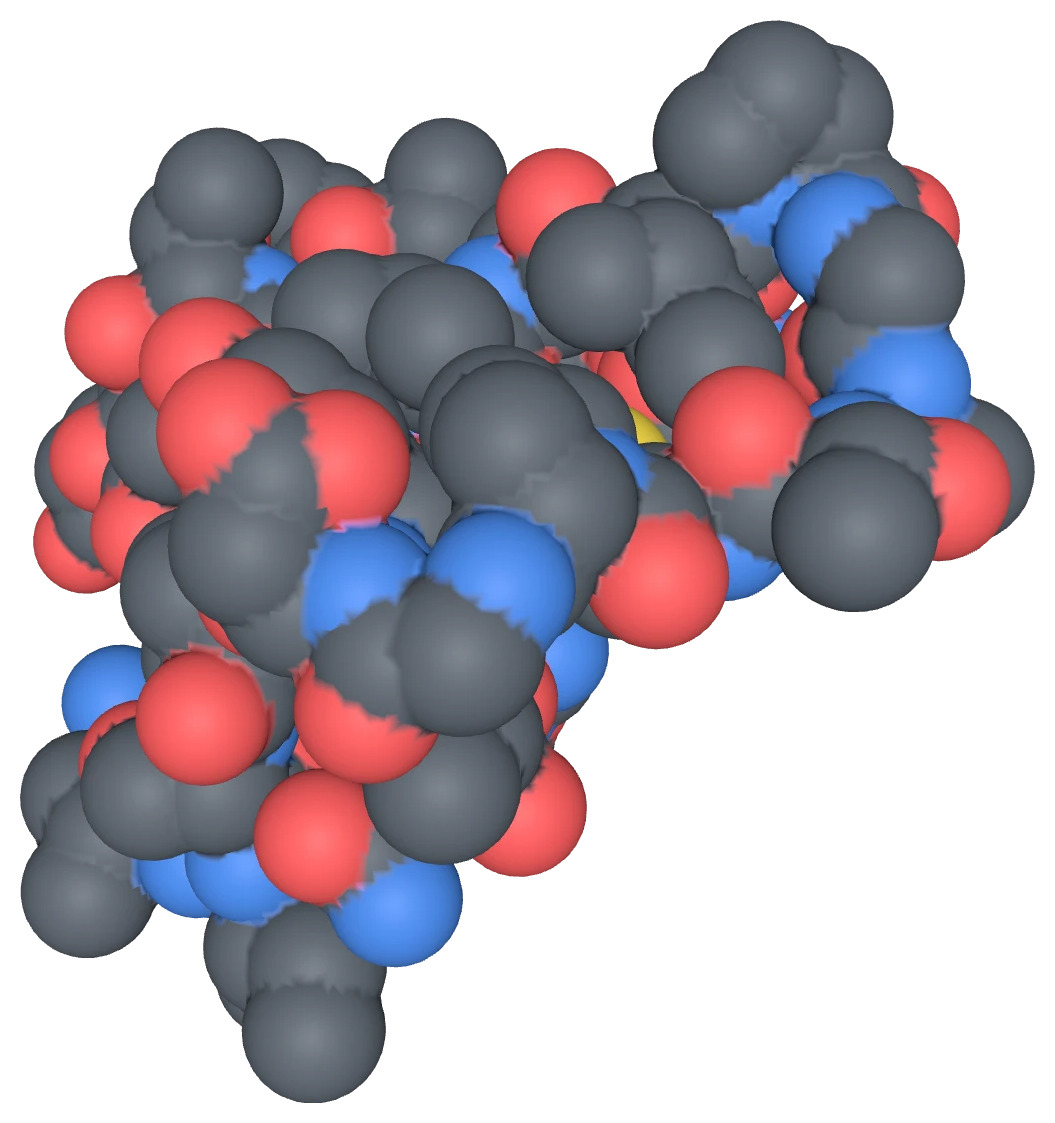
\includegraphics[width=\linewidth]{1crn-vdw}
    \caption{vdW surface}
  \end{subfigure}\hfill
  \begin{subfigure}[b]{0.32\linewidth}
    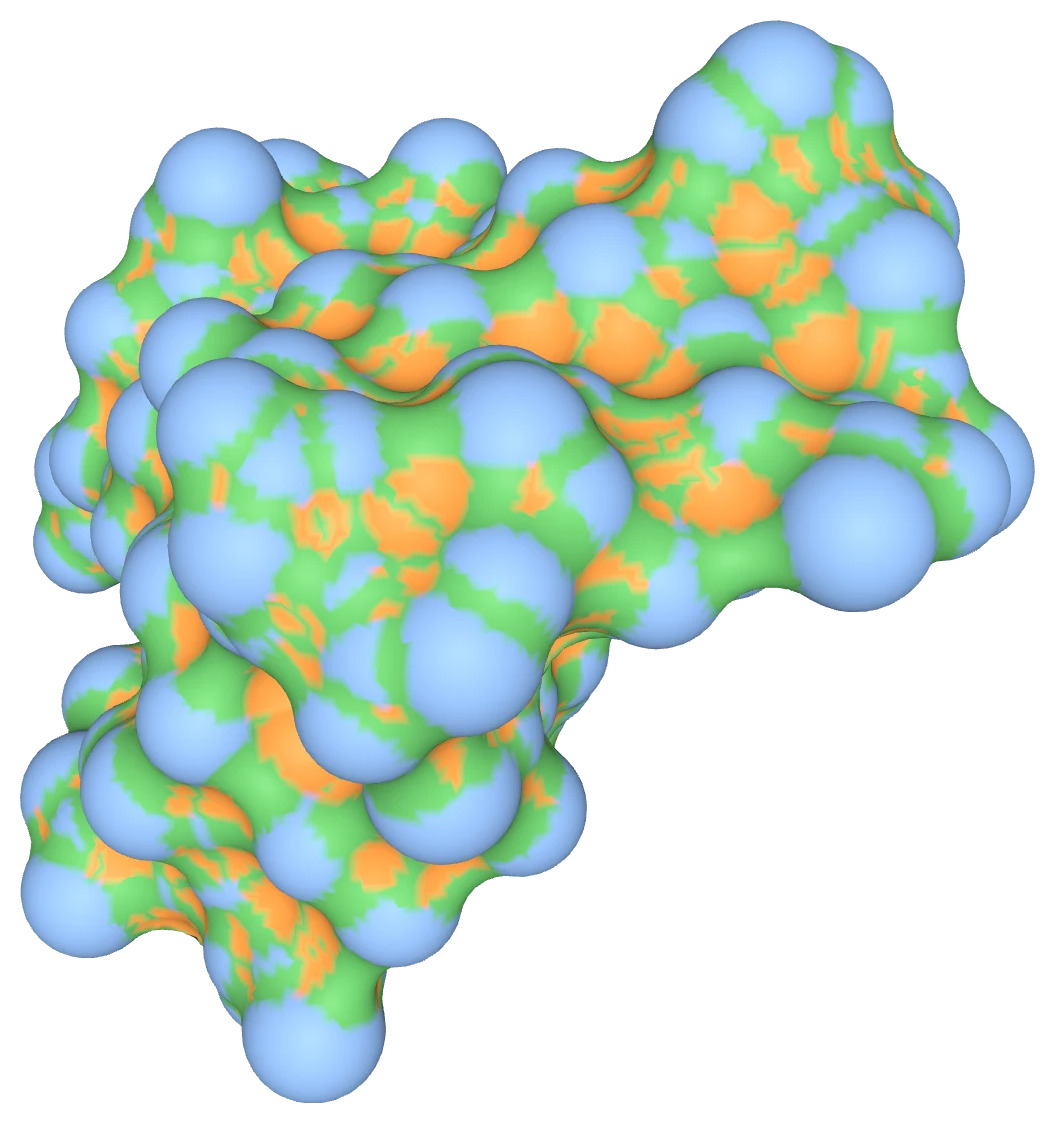
\includegraphics[width=\linewidth]{1crn-patch}
    \caption{SES, by patch type}
  \end{subfigure}\hfill
  \begin{subfigure}[b]{0.32\linewidth}
    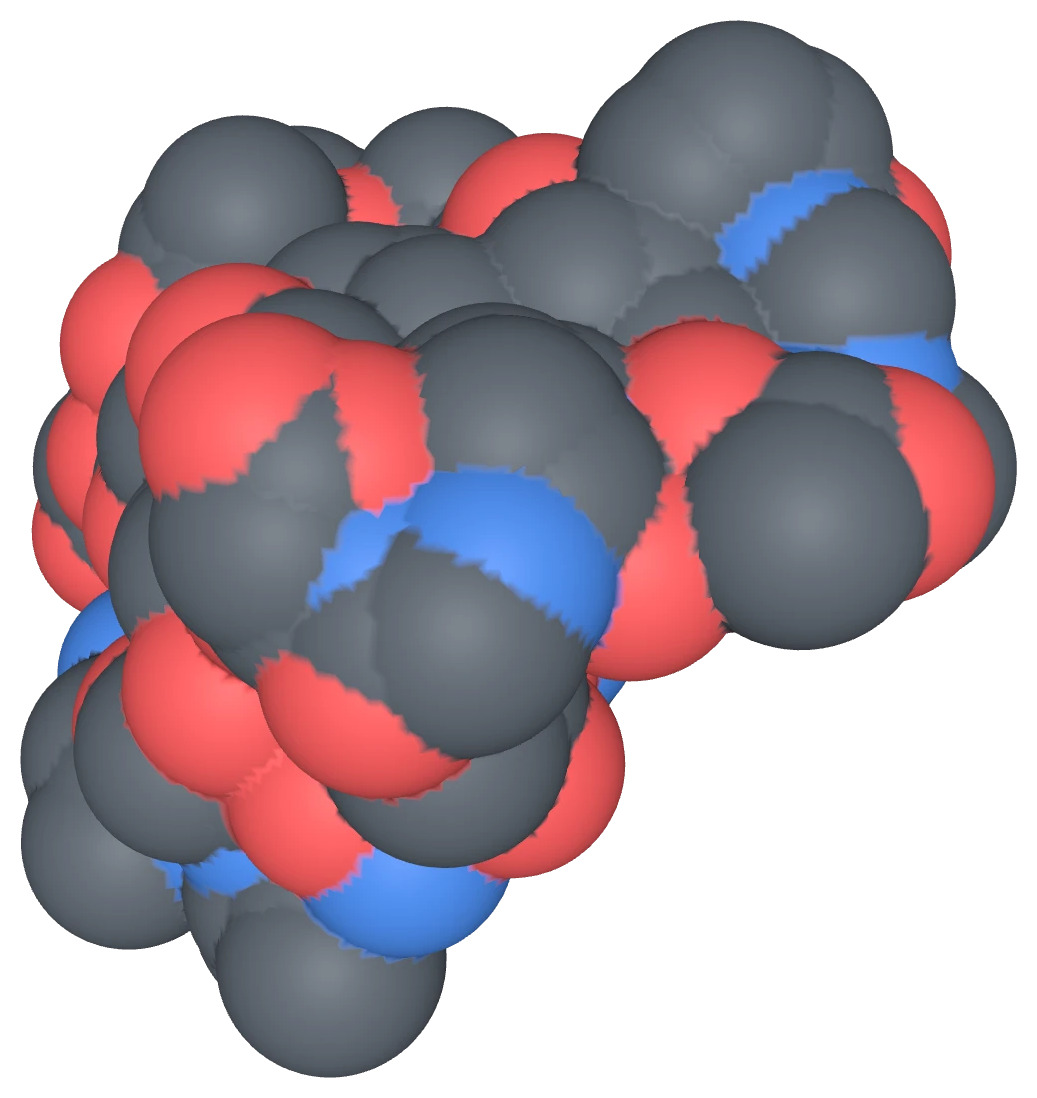
\includegraphics[width=\linewidth]{1crn-sas}
    \caption{SAS}
  \end{subfigure}
  \caption{The three surfaces of crambin (PDB 1CRN, 327 atoms) computed by
    \sesmesh{} at $h = 0.25$\Ang. (a)~vdW surface, coloured by element
    (198\,268 triangles). (b)~SES coloured by the patch type of each vertex:
    convex (blue), saddle (green), concave (orange). (c)~SAS, atom radii
    grown by $r_p = 1.4$\Ang. Renderings from the project website.}
  \label{fig:gallery-kinds}
\end{figure}

% sesmesh — Solvent Excluded Surface meshes for molecules
% Copyright (c) 2026 Ugo Varetto
% SPDX-License-Identifier: MIT OR Apache-2.0

\section{The SES as a level set}
\label{sec:background}

\paragraph{Definitions.}
Let atom $i = 1,\dots,N$ have centre $\vect c_i$ and radius $r_i > 0$, let
$r_p \ge 0$ be the probe radius and $R_i = r_i + r_p$ the expanded radii.
The open SAS solid is $A = \bigcup_i B^\circ(\vect c_i, R_i)$ and the SAS is
$\partial A$. The \emph{probe-accessible region}
\begin{equation}
  P = \mathbb R^3 \setminus A
    = \{\vect x : \norm{\vect x - \vect c_i} \ge R_i \ \forall i\}
\end{equation}
is the closed set of feasible probe centres. The \emph{excluded region}
$E = \{\vect x : d(\vect x, P) \ge r_p\}$ is the complement of the union of
all probe balls that do not overlap an atom~\cite{greer1978}, and the SES is
$\partial E$.

\paragraph{The SES field.}
\sesmesh{} samples
\begin{equation}
  F(\vect x) = r_p - d(\vect x, P),
  \label{eq:field}
\end{equation}
which is negative inside the molecule, positive in the solvent and zero on
the SES. Quan and Stamm~\cite{quan2016} showed that this level set is
exactly the SES, singularities included: self-intersecting tori and
intersecting concave patches are features of the level set of $F$ and need
no special treatment. The algorithm relies on six elementary properties
(proofs are short and given in the design document of the
repository):
\begin{enumerate}[label=(P\arabic*)]
  \item $F$ is 1-Lipschitz, as every distance function is.
    \label{p:lipschitz}
  \item $F(\vect x) = r_p$, its maximum, for $\vect x \in P$: everything
    outside the SAS is trivially ``outside''.
  \item Inside $E$, $|F(\vect x)| = \operatorname{dist}(\vect x, \mathrm{SES})$
    exactly; outside $E$, $0 < F(\vect x) \le \operatorname{dist}(\vect x,
    \mathrm{SES})$. \label{p:dist}
  \item $F(\vect x) \le s_{\mathrm{vdW}}(\vect x) :=
    \min_i(\norm{\vect x - \vect c_i} - r_i)$, because
    $d(\vect x, P) \ge R_i - \norm{\vect x - \vect c_i}$ for every $i$: a
    cheap ``inside'' test. \label{p:vdw}
  \item Where the closest point $\vect p(\vect x) \in P$ is unique and
    $\vect x \notin P$, $\nabla F(\vect x) = (\vect p - \vect x) /
    \norm{\vect p - \vect x}$; on the SES the outward unit normal is
    $\vect n = (\vect p - \vect x)/r_p$. \label{p:normal}
  \item For $\vect x \in E$, the point $\vect x^* = \vect p + r_p(\vect x -
    \vect p)/\norm{\vect x - \vect p}$ lies on the SES: an exact projection
    from inside. \label{p:project}
\end{enumerate}
The SAS and vdW surfaces use $F_{\mathrm{SAS}}(\vect x) =
\min_i(\norm{\vect x - \vect c_i} - R_i)$ and $F_{\mathrm{vdW}}(\vect x) =
\min_i(\norm{\vect x - \vect c_i} - r_i)$, which are also 1-Lipschitz and
exact on their zero sets; an SES with $r_p = 0$ is the vdW surface.

\paragraph{Closest point on the SAS.}
For $\vect x \in A$ the closest point of $P$ lies on $\partial A$, a union of
spherical faces, circular arcs (pairwise sphere intersections) and vertices
(triple intersections). It lies in the relative interior of a face or an
arc, or is a vertex; on a sphere the only interior local minimum of the
distance is the radial projection, on a circle the planar projection. Hence
$d(\vect x, P)$ is the minimum over three candidate classes, each subject to
a validity test---the candidate point must not lie strictly inside another
expanded sphere (\cref{tab:classes}). Class S produces the convex patches
of the SES, class C the saddles and class V the concave patches, so the
winning class of a vertex is its patch type.

\begin{table}[t]
  \centering
  \caption{Candidate closest points on the SAS for a query point $\vect x$.
    For circle $(i,j)$ with $D = \norm{\vect c_j - \vect c_i}$,
    $|R_i - R_j| < D < R_i + R_j$: $\vect u = (\vect c_j - \vect c_i)/D$,
    $t = (D^2 + R_i^2 - R_j^2)/(2D)$, centre $\vect m = \vect c_i + t\vect u$,
    radius $\rho = (R_i^2 - t^2)^{1/2}$; $\vect y = \vect x - \vect m$,
    $a = \vect y \cdot \vect u$, $\vect w = \vect y - a\vect u$. $N(i)$ is the
    set of spheres intersecting sphere $i$ and $K(i,j)$ the set of spheres
    that cut circle $(i,j)$.}
  \label{tab:classes}
  \small
  \begin{tabular}{@{}llll@{}}
    \toprule
    Class (SES patch) & Candidate $\vect q$ & Distance & Valid iff \\
    \midrule
    S, sphere $i$ (convex) &
      $\vect c_i + R_i \frac{\vect x - \vect c_i}{\norm{\vect x - \vect c_i}}$ &
      $\bigl|\norm{\vect x - \vect c_i} - R_i\bigr|$ &
      $\norm{\vect q - \vect c_k} \ge R_k\ \forall k \in N(i)$ \\[4pt]
    C, circle $(i,j)$ (saddle) &
      $\vect m + \rho\, \vect w/\norm{\vect w}$ &
      $\bigl(a^2 + (\norm{\vect w} - \rho)^2\bigr)^{1/2}$ &
      $\norm{\vect q - \vect c_k} \ge R_k\ \forall k \in K(i,j)$ \\[4pt]
    V, vertex $(i,j,k)$ (concave) &
      precomputed $\vect v$ & $\norm{\vect x - \vect v}$ &
      precomputed (exposed only) \\
    \bottomrule
  \end{tabular}
\end{table}

Degenerate queries have deterministic answers: at $\vect x = \vect c_i$
class S is undefined and skipped (the point is deep inside), and for
$\norm{\vect w} \approx 0$ all points of a circle are equidistant, so the
minimum over an exposed arc is attained at an arc endpoint (a class-V
vertex) or, for a fully exposed circle, at a fixed point. Validity uses
$\norm{\vect q - \vect c_k}^2 \ge R_k^2 - \tau_k$; a wrong decision for a
candidate within $\varepsilon$ of a blocking sphere changes the computed
distance by $O(\varepsilon)$, because the true closest point is then on the
nearby arc or vertex. Tolerances are therefore accuracy parameters, not
topology hazards; the only ill-posed inputs are exactly fitting probes,
which a fixed tolerance decides deterministically (\cref{sec:arrangement}).

\paragraph{Cavities.}
$P$ may have bounded components: probe-accessible pockets that the solvent
cannot reach from outside. Each yields closed SES components whose outward
normals point into the enclosed solvent, so they have negative signed
volume, while external components have positive signed volume. This gives
an exact and cheap classification on the mesh (\cref{sec:cavities}).

% sesmesh — Solvent Excluded Surface meshes for molecules
% Copyright (c) 2026 Ugo Varetto
% SPDX-License-Identifier: MIT OR Apache-2.0

\section{Method}
\label{sec:method}

The algorithm follows one principle: the surface is defined by the exact
function~\eqref{eq:field}; discretization decides only \emph{where} it is
sampled, never \emph{what} is computed. Vertices are roots of $F$ on grid
edges and normals are its exact gradient. \Cref{fig:pipeline} shows the
pipeline.

\begin{figure}[t]
  \centering
  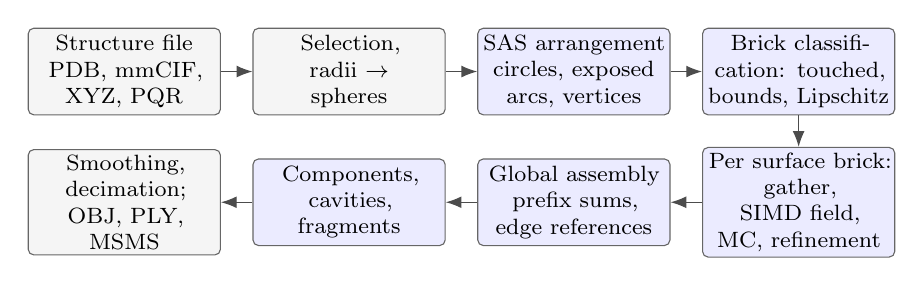
\begin{tikzpicture}[
      node distance=4mm and 4mm,
      box/.style={draw=black!60, rounded corners=2pt, fill=#1,
        align=center, font=\footnotesize, minimum height=11mm,
        text width=23mm, inner sep=2pt},
      box/.default=black!4,
      arr/.style={-{Latex[length=2mm]}, black!70}]
    \node[box] (in) {Structure file\\PDB, mmCIF,\\XYZ, PQR};
    \node[box, right=of in] (sel) {Selection,\\radii $\to$\\spheres};
    \node[box=blue!8, right=of sel] (arr) {SAS arrangement\\circles, exposed\\arcs, vertices};
    \node[box=blue!8, right=of arr] (cls) {Brick classifi-\\cation: touched,\\bounds, Lipschitz};
    \node[box=blue!8, below=of cls] (mesh) {Per surface brick:\\gather, SIMD field,\\MC, refinement};
    \node[box=blue!8, left=of mesh] (asm) {Global assembly\\prefix sums,\\edge references};
    \node[box=blue!8, left=of asm] (post) {Components,\\cavities,\\fragments};
    \node[box, left=of post] (out) {Smoothing,\\decimation;\\OBJ, PLY, MSMS};
    \draw[arr] (in) -- (sel); \draw[arr] (sel) -- (arr);
    \draw[arr] (arr) -- (cls); \draw[arr] (cls) -- (mesh);
    \draw[arr] (mesh) -- (asm); \draw[arr] (asm) -- (post);
    \draw[arr] (post) -- (out);
  \end{tikzpicture}
  \caption{Pipeline. Shaded stages form the surface core, which takes
    spheres and returns a mesh; parsing, radii and export are layers around
    it. Every stage after parsing runs in parallel and produces the same
    result for any number of threads.}
  \label{fig:pipeline}
\end{figure}

\subsection{The SAS arrangement}
\label{sec:arrangement}

All geometric constructions use 64-bit floating point. Spheres with
$R_i = 0$ are removed and exact duplicates (same centre within
$10^{-9}$\Ang{} and same radius) are collapsed. Spheres are sorted by the
Morton code of their cell for locality, and a uniform cell list with cell
size $2\max_i R_i$ (about 6.4\Ang{} for proteins with $r_p = 1.4$\Ang),
built by counting sort, answers range queries; very sparse inputs double the
cell size until the grid has at most $\max(65\,536, 8N)$ cells.

A sphere lying inside another is marked \emph{contained} and ignored.
For every intersecting pair $(i,j)$ a circle frame
$(\vect m, \vect u, \vect e_1, \vect e_2, \rho)$ is built. For each common
neighbour $k$, the points of circle $(i,j)$ inside ball $k$ form an angular
interval: with $\vect g = \vect m - \vect c_k$,
$\norm{\vect q(\theta) - \vect c_k}^2 = \norm{\vect g}^2 + \rho^2 +
2\rho(\cos\theta\, \vect e_1\cdot\vect g + \sin\theta\, \vect e_2\cdot\vect g)
< R_k^2$, i.e.\ $\cos(\theta - \varphi_k) < \beta_k$, which is empty, the
full circle, or an interval centred at $\varphi_k + \pi$. Endpoints are
computed as unit vectors with angle-addition formulas, and intervals are
sorted and merged on a monotone, trigonometry-free pseudo-angle; this made
the circle stage about $1.8\times$ faster on GroEL--GroES (PDB 1AON). A
circle covered completely is \emph{buried} and discarded; otherwise its
blockers $K(i,j)$ are the spheres with non-empty intervals. The endpoints of
exposed arcs are the SAS vertices---probe positions touching three atoms,
the vertices of the reduced surface of MSMS~\cite{sanner1996}. Each triple
$i < j < k$ is enumerated exactly once, from exposed circle $(i,j)$ and
blocker $k > j$, and kept if no other neighbour of $i$ contains it, a single
source of truth independent of how the arcs were merged. A sphere is
\emph{exposed} if it has no neighbour or at least one exposed circle; a
buried sphere still blocks but never yields a class-S candidate. Containment,
intersection and strict-inclusion tests use an absolute tolerance of
$10^{-9}$\Ang, which decides exactly fitting probes deterministically;
symmetric lattices, icosahedral and dodecahedral cages, collinear chains and
exact duplicates are covered by tests (\cref{sec:robustness}).

The cost is $O(N\bar k^2)$ for $\bar k$ neighbours per atom, dominated by
about 20 blocker tests for each of about 20 candidate circles per atom.
Single-threaded, the arrangement took 3.3\,ms for crambin (1CRN), 56\,ms for
haemoglobin (4HHB), 0.73\,s for 1AON (59\,k atoms) and 3.0\,s for the 80S
ribosome 4V6X (238\,k atoms) when it was first built; it now runs in
parallel per sphere.

\subsection{Sparse narrow-band brick lattice}
\label{sec:lattice}

\paragraph{Lattice and bricks.}
Samples lie on the lattice $\vect o + h\,(i,j,k)$, $i,j,k \in \mathbb Z$,
where the frame origin $\vect o$ is the centre of the bounding box rounded
to a multiple of $h$, so the lattice coincides with multiples of $h$ in
input coordinates and kernel coordinates stay small. A \emph{brick} is a
block of $B^3$ cells ($B = 10$ by default; it was measured 4--10\,\%
faster end to end than $B = 8$ on 4HHB and 1AON, while 4, 6, 14 and 16 were
slower). Each brick evaluates its own $(B+1)^3$ samples, an apron that
includes its upper faces, so bricks are independent work items; the
duplicated samples ($1.33\times$ at $B = 10$) buy freedom from
synchronization between bricks.

\paragraph{Clamped field.}
Exact values are needed only near the surface. With the band
$\delta = \sqrt3\,h$, \sesmesh{} evaluates
$\tilde F = r_p - \min\bigl(d(\vect x, P),\, r_p + \delta\bigr)$, which is
exact wherever $|F| \le \delta$, has the correct sign everywhere and is
still 1-Lipschitz. Distances beyond $D = r_p + \delta$ are never needed,
which bounds every candidate search.

\paragraph{Conservative classification.}
Let $\vect b$ be a brick centre, $\rho_b = \tfrac{\sqrt3}{2}Bh$ its
circumradius and $\varepsilon_c = 2\cdot10^{-3}$\Ang{} a margin above the
kernel's rounding error (\cref{sec:kernel}). Then:
\begin{enumerate}
  \item \emph{Touched set.} Bricks overlapping no ball
    $B(\vect c_i, R_i + \varepsilon_c)$ lie in $P$ and are uniformly
    outside; they are never enumerated. Every sphere marks the bricks it
    overlaps, in a dense bitset when the brick lattice has at most $2^{31}$
    bricks and by a parallel sort and deduplication of brick keys
    otherwise.
  \item \emph{Cheap bounds} from nearest-sphere queries:
    $s_{\mathrm{SAS}}(\vect b) \ge \rho_b + \varepsilon_c$ means the brick
    lies in $P$ (uniformly outside), and
    $s_{\mathrm{vdW}}(\vect b) \le -(\rho_b + \varepsilon_c)$ means it is
    uniformly inside, by~\ref{p:vdw}.
  \item \emph{Lipschitz test.} If
    $|\tilde F(\vect b)| > \rho_b + \varepsilon_c$, the brick is uniform
    with the sign of $\tilde F(\vect b)$, by~\ref{p:lipschitz}.
  \item Otherwise it is a \emph{surface brick}.
\end{enumerate}
Uniform bricks produce no geometry. This is the adaptive distance field
idea~\cite{frisken2000} and the brick culling of Hermosilla et
al.~\cite{hermosilla2017}, made exact by the Lipschitz bound. The same test
classifies the $2^3$ sub-blocks of each surface brick: samples that lie only
in uniform sub-blocks receive the value $\pm\delta$ (exact sign, inexact
value) without evaluation. Meshing needs exact values only at both ends of
sign-changing edges, which never touch a uniform sub-block, so this changes
no vertex. On 1AON about 23\,\% of samples are culled this way at
$h = 0.5$\Ang{} and about 56\,\% at $0.25$\Ang.

\paragraph{Candidate gathering.}
Candidates are gathered per active sub-block (centre $\vect b$,
circumradius $\rho$) within $G = r_p + \delta + \rho$ of $\vect b$ into
reusable thread-local structure-of-arrays buffers: the non-contained
spheres that can block (those that can contain a sample first, as only
they are scanned by the inside-SAS test), class-S candidates sorted by
distance (nearest first, for better pruning) with their blockers within
reach, class-C candidates with filtered blocker lists, and class-V
vertices within $G$. Any candidate that can be the closest point (at
distance $\le D$) of a sample in the sub-block lies within $G$ of
$\vect b$, and any sphere that can invalidate it contains a point within
$G$ of $\vect b$; the gathered sets therefore give the same minimum as the
global ones.

\subsection{Vectorized field kernel}
\label{sec:kernel}

SIMD lanes map to samples. The active samples of a sub-block are compacted
into 32-bit floating-point coordinate arrays, computed in the centred frame
from integer lattice indices and padded to a multiple of 16, so there is no
scalar tail. Vectors hold eight lanes (one AVX2 register, or two NEON
registers, which measured about 10\,\% faster than native four-lane NEON on
1AON thanks to the extra instruction-level parallelism). Per vector, the
kernel keeps the squared best distance, initialized to $D^2$, and processes
(1)~class-V vertices with one minimum per vertex; (2)~class-S candidates,
skipping a candidate when the lower bound
$\bigl|\norm{\vect x - \vect c} - R\bigr|$ improves no lane, otherwise
computing the candidate points, AND-reducing validity over the blockers
with an early exit once all active lanes are invalid, and updating the
minimum under a mask; (3)~class-C candidates in the same way. The output is
$\tilde F = r_p - \sqrt{\text{best}^2}$. On 4HHB at $h = 0.5$\Ang{} a
sub-block of $4^3$ cells evaluates about 96 samples against about 10
``inside'' spheres, 23 class-S candidates (19 blockers each), 41 class-C
candidates (11 blockers each) and 12 class-V vertices; validity tests
dominate.

\paragraph{Precision and seams.}
Kernel arithmetic is single precision in the centred frame. Differences of
nearby coordinates are exact (Sterbenz lemma), so the error is dominated
by input rounding, about $3\cdot10^{-5}$\Ang{} for coordinates up to
500\Ang{} from the origin; if any coordinate would lie more than 2\,000\Ang{}
from the frame origin, the engine evaluates samples with the exact
double-precision evaluator instead. Neighbouring bricks must agree on the
sign of every shared sample. An evaluated sample uses identical inputs in
every brick (position from integers, identical feature data, the same
instruction sequence and SIMD level, padded tails), every gathered set
contains all candidates that can win or invalidate, and skipping by lower
bound never changes the minimum, so evaluated values are bit-identical. A
sample that is sign-only in one brick has the exact sign, and the kernel's
error (below $10^{-4}$\Ang) is far below the classification margin
$\varepsilon_c$. Tests check every seam of random clusters and of crambin.

\subsection{Marching Cubes with a uniform face rule}
\label{sec:mc}

A lattice corner is \emph{inside} iff $\tilde F < 0$; zero counts as
outside, one rule everywhere. Cells are triangulated with a 256-case
Marching Cubes table~\cite{lorensen1987} whose ambiguous faces always
separate the inside corners. Because the rule depends only on the face,
adjacent cells agree on every shared face, which makes the output
crack-free, closed and edge-manifold. The table is generated by a
test-only program: per face, the rule gives oriented segments (inside on a
fixed side), which chain into loops per cell; each loop receives, among
\emph{all} its triangulations, one that (0)~has no diagonal joining two
vertices of the same cube face, since the neighbouring cell could produce
the same edge and four triangles would share it (this was found on 4HHB),
(1)~has no vertex whose area-weighted normal points from the outside end of
its edge to the inside end, (2)~has the least area (no folds) and (3)~has
the largest minimum angle. Tests check that the generator reproduces the
table, that every case uses exactly its crossing edges, that all
$3 \times 256 \times 16$ shared-face pairings match with opposite
orientations, that interior edges never lie in a face, and that the winding
is outward. Rows of cells without a sign change are skipped early, the
trimming idea of Flying Edges~\cite{schroeder2015}. The uniform rule does
not reproduce the topology of the trilinear interpolant in ambiguous cells
as MC33 does~\cite{lewiner2003,custodio2013}; it is chosen for guaranteed
manifoldness, and the topology converges as $h$ decreases.

\paragraph{Edge ownership.}
An edge is keyed by its lower sample and axis. A brick \emph{owns} the
edges whose lower sample lies in its half-open range $[0,B)^3$; edges on
its upper faces belong to the neighbours. A neighbour owning an edge with a
sign change is necessarily a surface brick, because a uniform brick has a
guaranteed uniform sign on its closed region, so cross-brick references
always resolve. The converse fails: a surface brick may own no crossing edge
and still contain crossing cells, whose crossings all lie on its upper
faces, so the cell pass runs for every surface brick (an early version
that skipped such bricks left holes).

\subsection{Exact vertices, analytic normals and attributes}
\label{sec:refine}

Each owned crossing edge, in ascending local edge order, creates one vertex.
Starting from the linear estimate $t_0 = \tilde F_a/(\tilde F_a - \tilde F_b)$,
the root of $g(t) = F(\vect a + t(\vect b - \vect a))$ is refined with a
safeguarded Newton iteration: the closest point of each evaluation gives
the exact gradient, of unit length, so one step from the linear guess
usually lands within tolerance; steps that leave the bracket fall back to
the Illinois method and then to bisection. With a tolerance of
$10^{-5}$\Ang{} and at most eight evaluations, refinement needs 2.2--2.5
field evaluations per vertex (pure Illinois needed 3.2--3.6). Evaluations
are scalar double precision against per-sub-block candidate lists whose
blockers are restricted to the spheres within reach; one evaluation costs
about 0.5\,\textmu s, about the SIMD kernel's cost per sample, so a
vectorized single-precision refinement would save little while losing
exact vertices.

The parameter is clamped to $t \in [10^{-4}, 1 - 10^{-4}]$ so that
vertices from edges meeting at a sample with $F \approx 0$ never coincide,
which excludes zero-area triangles; the induced error is at most
$10^{-4}h$. The clamp distance is also at least four single-precision ulps
of the largest coordinate, so the separation survives the 32-bit output
positions; it stays below $2.4\cdot10^{-4}$\Ang{} for coordinates up to
1\,000\Ang. (The ulp condition was added after a test 10\,000\Ang{} from
the origin collapsed two vertices into one 32-bit value.)

The final evaluation's closest point $\vect p$ gives the analytic normal
$\vect n = (\vect p - \vect v)/\norm{\vect p - \vect v}$ by~\ref{p:normal},
the patch type from the winning candidate class (S convex, C saddle, V
concave) and the nearest atom as the argmin of
$\norm{\vect v - \vect c} - r$ over the atoms generating that feature, the
``closest sphere'' semantics of MSMS~\cite{sanner1996}. For the SAS and vdW
surfaces the normal is the radial direction of the active sphere. A
cheaper \code{linear} mode skips refinement for previews.

\subsection{Deterministic global assembly}
\label{sec:assembly}

Each brick, in parallel, emits its triangles as references
(owning neighbour, local edge id) and stores its owned crossing edges as an
array sorted by edge id. A prefix sum of vertex counts over the sorted
brick list gives each brick's first global vertex; positions, normals and
attributes are concatenated in brick order; references are then resolved
in parallel by binary search in the owner's edge array. The output order
depends only on the brick order, the edge ids and the cell order, never on
scheduling. Every mesh is validated before it is returned---each undirected
edge used by exactly two triangles in opposite directions, no degenerate or
duplicate triangles, finite coordinates---and a violation is reported as an
internal error rather than written.

\subsection{Components, cavities and enclosure}
\label{sec:cavities}

Components are found by union--find over vertices along triangle edges.
Links always go from the larger root to the smaller, so the partition and
its labelling by smallest vertex index do not depend on the schedule even
with a lock-free parallel implementation. For each component, \sesmesh{}
computes in fixed-order double-precision sums the area, the signed volume
$\sum \vect v_0 \cdot (\vect v_1 \times \vect v_2)/6$, the Euler
characteristic $\chi = V - E + F$ and the genus $(2 - \chi)/2$.

Components with negative signed volume are cavities (\cref{sec:background}).
Three modes are offered: \code{keep} (the default: the exact SES including
cavities), \code{remove} (drop the cavities, as MSMS reports only the
external surface by default~\cite{msmsmanual}) and \code{only}. Removing a
cavity also removes every positive component inside it---a molecule
fragment enclosed in a pocket---found by a ray-parity point-in-mesh test of
one vertex after a bounding-box test. Filters by minimum cavity volume and
minimum component area apply in every mode. Triangles are reordered so that
each component is contiguous (for per-component groups in OBJ output).
Removing cavity components equals computing the SES of the unbounded
component of $P$ only, except in the degenerate case where a cavity's probe
balls touch external probe balls; both then belong to the same mesh
component and are kept.

\subsection{Sub-grid fragments}
\label{sec:fragments}

Where the solid side of the SES is a sheet thinner than $h$, Marching Cubes
can cut off small solid components that are not separate in the exact
surface. The typical case is two probe positions touching the same three
atoms from opposite sides of their plane, at a height just below $r_p$: the
SES spans the atom triangle with a sheet around a pinhole, its thickness
going to zero at the hole. In 4HHB at $h = 0.25$\Ang{} one such sheet
(atoms O1D of HEM~D148, OG of SER~D44 and CE2 of PHE~D45; probe height
1.371\Ang, pinhole radius 0.283\Ang) is 0.069\Ang{} thick at one lattice
node, where $F = -0.0049$\Ang, while its six neighbours are outside
($F = +0.025$ to $+0.219$\Ang); Marching Cubes emits an isolated octahedron
of 8 triangles and 0.037\AA$^2$ whose vertices are all concave. A flood
fill on a 0.01\Ang{} grid through $F < 0$ reaches the CE2 atom after
1.1\Ang: in the exact SES the sheet belongs to the main body.

Every true solid component contains an atom ball and its extreme points in
every direction lie on convex patches, so it has convex area of the order of
$4\pi R^2$. \sesmesh{} therefore defines a \emph{sub-grid fragment} as a
non-cavity component without any convex vertex; cavities contain a whole
probe ball (at least 11.5\AA$^3$ for $r_p = 1.4$\Ang) and are never
fragments. Fragments are dropped on request (\code{--drop-fragments}); the
option is off by default in the 1.x series so that default output stays
byte-identical to 1.0. \Cref{tab:fragments} shows that fragments are tiny
and well separated from the smallest true solid components. Finer grids
place more nodes in thin sheets (4HHB has 0, 2, 2, 1, 5 and 7 fragments at
$h = 0.5$, 0.35, 0.3, 0.25, 0.2 and 0.15\Ang) while each fragment's area
shrinks as $h^2$.

\begin{table}[t]
  \centering
  \caption{Sub-grid fragments in the validation corpus
    (\val{corpus-n} entries, Bondi radii, $r_p = 1.4$\Ang), counted with
    \sesmesh{} 1.1.0 (design document \S9.1). ``Triangles'' gives how many
    fragments have 8, 16, 24 or 32 triangles. On the \val{sweep-n}-entry
    sweep set at $h = 0.5$\Ang: 1\,026 fragments in 119 entries, the largest
    2.66\AA$^2$, the smallest true solid component 36.5\AA$^2$.}
  \label{tab:fragments}
  \small
  \begin{tabular}{@{}rrrlrr@{}}
    \toprule
    $h$ (\AA) & Fragments & Entries & Triangles 8/16/24/32 &
      Largest (\AA$^2$) & Smallest true solid (\AA$^2$) \\
    \midrule
    1.0  & 100   & 12 & 98/2/0/0       & 3.00 & 37.7 \\
    0.7  & 237   & 18 & 235/1/1/0      & 2.48 & 39.3 \\
    0.5  & 512   & 27 & 499/12/1/0     & 1.91 & 40.0 \\
    0.35 & 851   & 31 & 816/32/3/0     & 0.84 & 40.3 \\
    0.25 & 1\,358 & 36 & 1\,273/75/7/3 & 0.54 & 40.5 \\
    \bottomrule
  \end{tabular}
\end{table}

\subsection{Level of detail}
\label{sec:lod}

\paragraph{Spacing, presets and vertex density.}
The grid spacing $h$ is the primary control, with presets \code{draft}
(1.0\Ang), \code{low} (0.7\Ang), \code{medium} (0.5\Ang, the default, as in
ChimeraX~\cite{chimeraxsurface}), \code{high} (0.25\Ang) and \code{ultra}
(0.1\Ang). Users of MSMS think in vertices per \AA$^2$; for Marching Cubes
on a smooth surface with unit normal $\vect n$, the number of crossing
edges per unit area is about $(|n_x| + |n_y| + |n_z|)/h^2$, whose average
over uniformly distributed orientations is $1.5/h^2$. A requested density
$d$ is therefore mapped to $h = \sqrt{1.5/d}$; \cref{sec:density} confirms
the constant.

\paragraph{Smoothing with exact re-projection.}
Marching Cubes produces slivers where the surface nearly passes through
lattice nodes. Optional Taubin $\lambda|\mu$ smoothing~\cite{taubin1995}
($\lambda = 0.5$, $\mu = -0.53$, uniform umbrella Laplacian, parallel
Jacobi updates) is followed by re-projection of every vertex,
$\vect x \leftarrow \vect x - F(\vect x)\nabla F(\vect x)$, exact in one
step from inside $E$ by~\ref{p:project} (at most four steps), and by
recomputation of normals and attributes. In the tests, vertices stay within
$10^{-4}$\Ang{} of the SES after five rounds, the number of triangles with a
minimum angle below $10^\circ$ is more than halved and the area changes by
less than 1\,\%.

\paragraph{Decimation.}
Decimation uses Garland--Heckbert plane quadrics~\cite{garland1997} with
\emph{half-edge} collapses $u \to v$ only, so no new positions are created
and every retained vertex keeps its exact position, analytic normal, atom
and patch type. Instead of a global priority queue, each pass builds one
candidate per live edge (the cheaper direction, if its error is below the
bound), sorts the candidates in parallel with ties broken by vertex index
(so the result is deterministic) and applies them in order, skipping a
candidate whose endpoints' one-rings were already touched in that pass;
passes repeat until the target is met or nothing collapses. A collapse is
applied only if both endpoints share exactly two triangles, the link
condition holds, no triangle normal turns by more than about $78^\circ$, no
new triangle has a quality below 0.05 and the component keeps more than
four triangles. The mesh is then compacted and validated again. Crambin at
$h = 0.25$\Ang{} goes from 111\,076 to 27\,768 triangles in about 120\,ms;
on 1AON at 0.25\Ang{} the passes take about 6.5\,s where a heap with
re-queued edges took about 20\,s. Decimating a fine mesh concentrates
triangles where the surface bends (\cref{fig:lod}).

\begin{figure}[t]
  \centering
  \begin{subfigure}[b]{0.49\linewidth}
    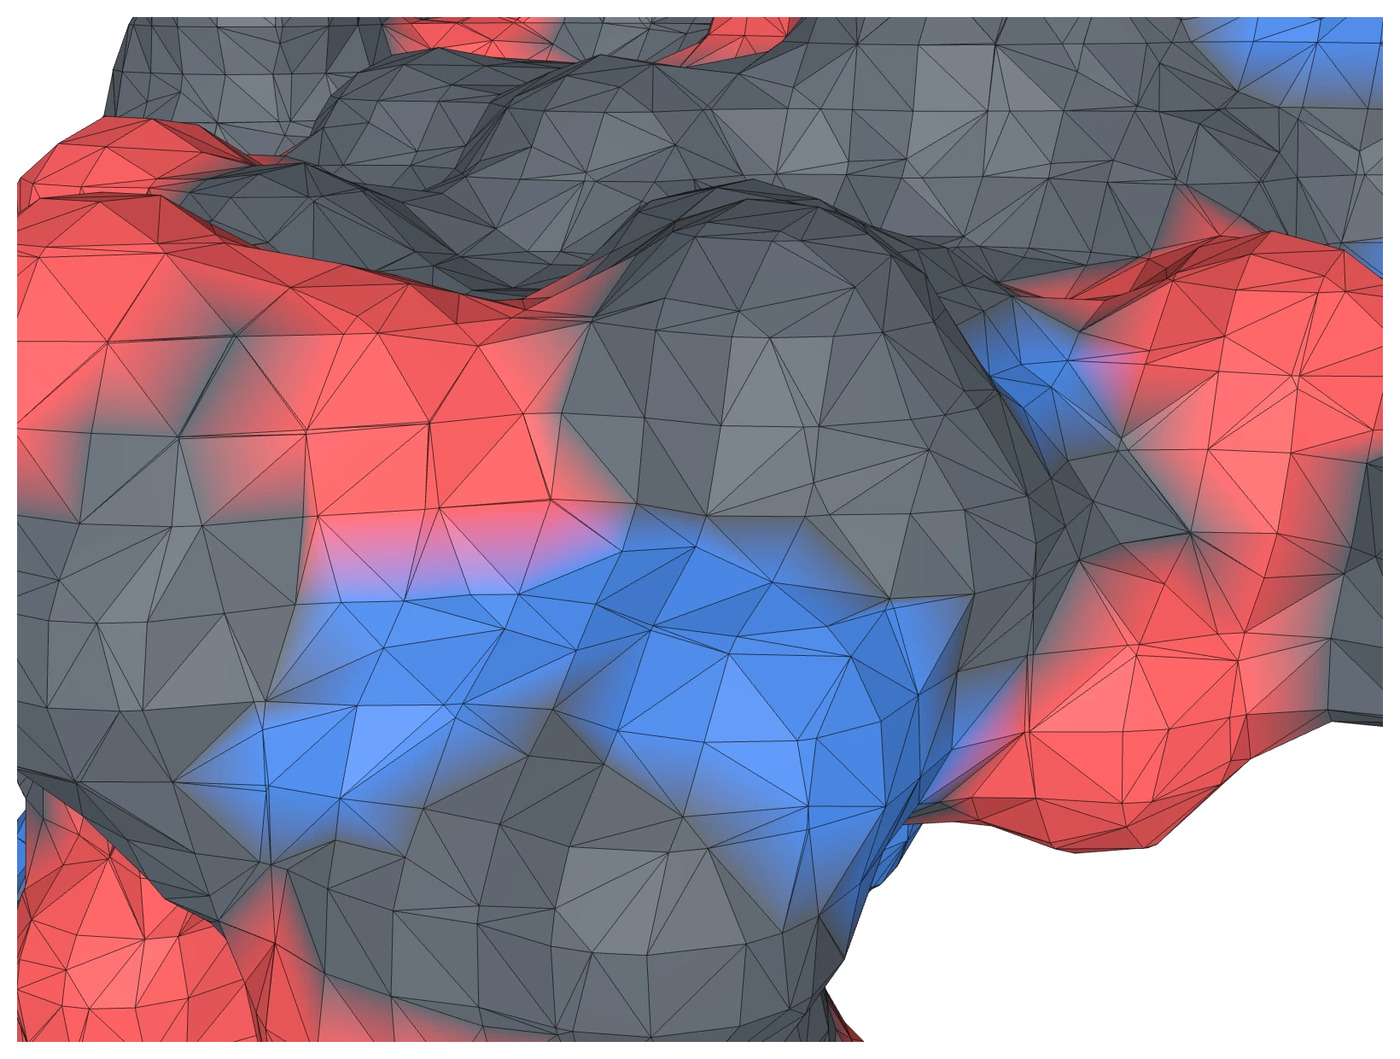
\includegraphics[width=\linewidth]{1crn-coarse}
    \caption{$h = 0.7$\Ang, 13\,996 triangles}
  \end{subfigure}\hfill
  \begin{subfigure}[b]{0.49\linewidth}
    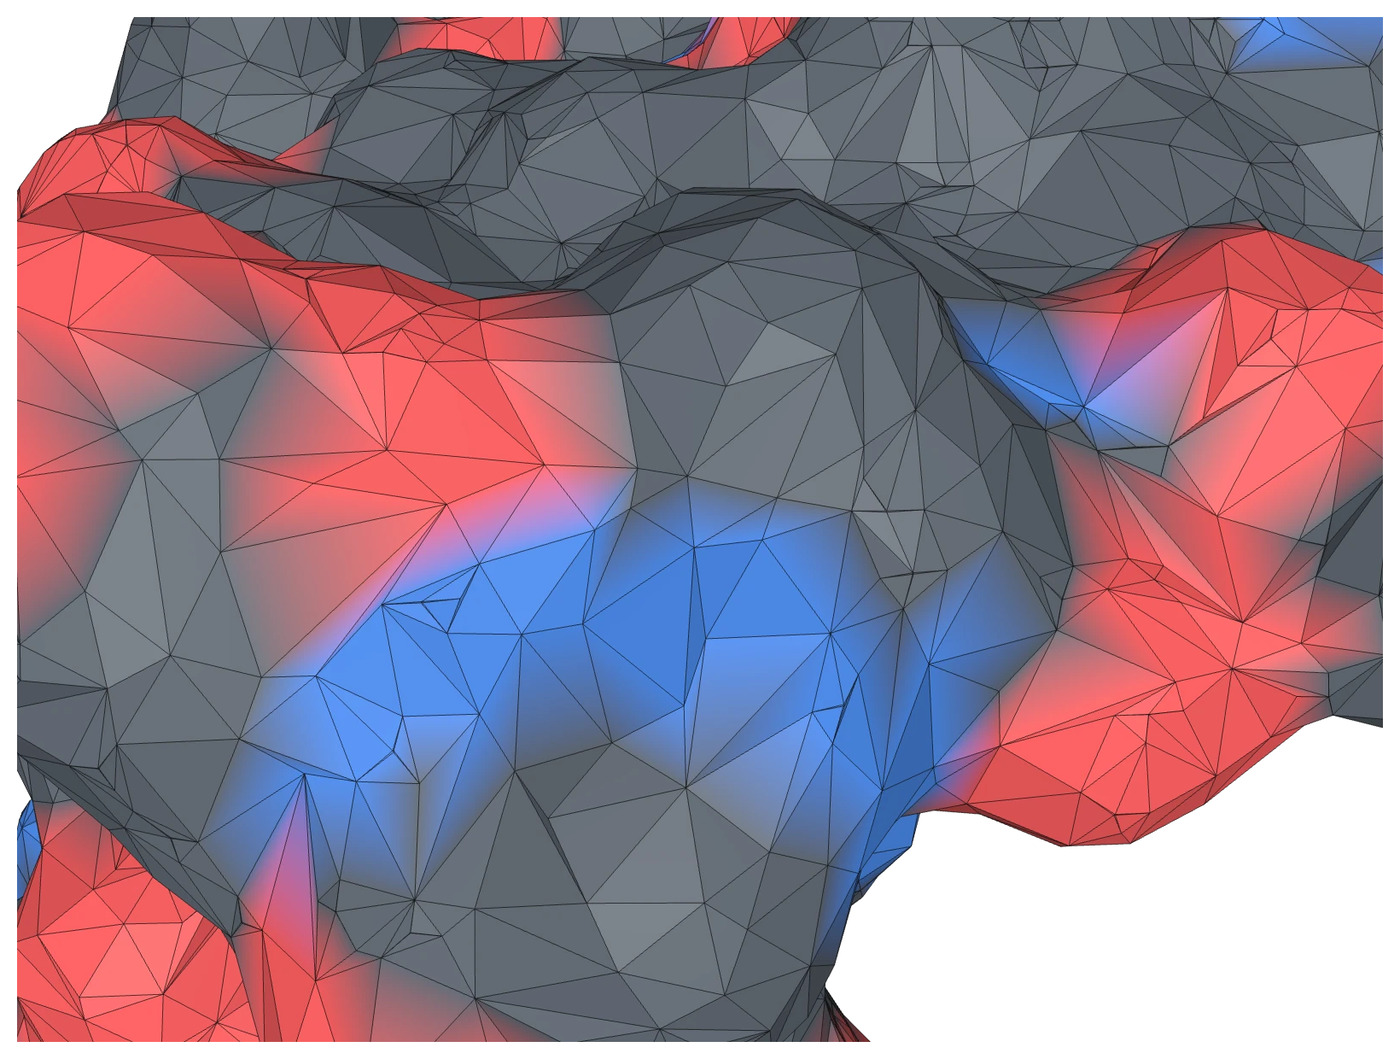
\includegraphics[width=\linewidth]{1crn-decimated}
    \caption{$h = 0.25$\Ang{} decimated to 13\,996 triangles}
  \end{subfigure}
  \caption{Two ways to spend the same triangle budget on crambin, coloured
    by element. (a)~A coarse grid gives uniform triangles everywhere.
    (b)~Decimating a fine mesh gives large triangles where the surface is
    flat and small ones where it bends; every vertex is still on the exact
    SES.}
  \label{fig:lod}
\end{figure}

% sesmesh — Solvent Excluded Surface meshes for molecules
% Copyright (c) 2026 Ugo Varetto
% SPDX-License-Identifier: MIT OR Apache-2.0

\section{Implementation}
\label{sec:implementation}

\sesmesh{} is written in Rust (edition 2024, minimum supported compiler
1.89) as a Cargo workspace of a library crate, \code{sesmesh}, a
command-line crate, \code{sesmesh-cli} (binary \code{sesmesh}), and a
development-only crate of test oracles, analytic references and cluster
generators. All crates forbid \code{unsafe} code, every public item is
documented, the library never prints (warnings are returned as values), and
the public API exposes no third-party types, so dependency upgrades cannot
break callers. Since 1.0 the project follows semantic versioning, and the
1.x series keeps the default output byte-identical; new behaviour is
opt-in.

\subsection{Library and command-line interface}

The core entry point takes spheres and parameters and returns a mesh with
per-vertex normals, nearest atoms, patch types and components, plus
statistics; structure readers, atom selection and radius assignment are
separate composable functions (\cref{lst:api}). A reusable
\code{SurfaceEngine} keeps per-thread buffers between calls for
trajectories, and a \code{Control} object carries a cancellation flag and a
progress callback; cancellation is checked per sphere, between stages and
per brick, and takes effect within one brick's work (under 100\,ms in the
tests). The command-line tool exposes every library option, writes one or
many inputs (batch mode with per-file error isolation), reports timings and
statistics, generates shell completions and a manual page, and uses
distinct exit codes (0 success, 1 runtime error, 2 usage error, 3 input
parse error, 4 resource limit, 130 interrupted).

\begin{figure}[t]
\begin{lstlisting}[language=Rust]
use sesmesh::export::obj::{write_obj_path, ObjOptions};
use sesmesh::{compute_surface, io, radii, Diagnostics, Selection, Sphere, SurfaceParams};

fn main() -> sesmesh::Result<()> {
    let structure = io::read_path("1crn.cif", &io::ReadOptions::default())?;
    let mut diags = Diagnostics::new();
    let atoms = structure.select(&Selection::default(), &mut diags)?;
    let radii = radii::assign(&atoms, &radii::RadiusOptions::default(), &mut diags)?;
    let spheres = Sphere::from_atoms(&atoms, &radii)?;
    let out = compute_surface(&spheres, &SurfaceParams::ses(1.4).with_spacing(0.25))?;
    println!("{} triangles, area {:.1} A^2", out.stats.triangles, out.stats.area);
    write_obj_path("1crn.obj", &out.mesh, &ObjOptions::default())
}
\end{lstlisting}
\begin{lstlisting}
sesmesh 1crn.cif -q high --cavities remove --vertex-colors element --stats stats.json
sesmesh 1k4r.cif.gz --assembly 1 -q draft -o capsid.ply      # 545k-atom capsid
sesmesh 3j3q.cif.gz --max-memory 4G --auto-coarsen          # coarsen until it fits
\end{lstlisting}
  \caption{Library use (from the README; the snippets on the project
    website are compiled against 1.1.0) and three command-line
    invocations.}
  \label{lst:api}
\end{figure}

\paragraph{Inputs.}
Purpose-built readers parse PDB (fixed columns, hybrid-36 serial
numbers~\cite{pdbformat33,hybrid36}, chunked parallel parsing of large
files), PDBx/mmCIF~\cite{mmcif} (a full CIF~1.1 lexer and the
\code{\_atom\_site} loop in any column order; about 350\,MiB/s on one core;
the gzipped 2.44-million-atom 3J3Q entry reads in about 0.8\,s), XYZ
and extended XYZ~\cite{extxyz}, and PQR~\cite{pqr}, each optionally gzip
compressed~\cite{flate2}. Biological assemblies are generated from mmCIF
\code{pdbx\_struct\_\allowbreak assembly\_gen} and
\code{pdbx\_struct\_\allowbreak oper\_list} and PDB
\code{REMARK 350}; the 1K4R entry contains 9\,084 deposited atoms of a
capsid of 545\,040. Assemblies of more than 100\,000 copies or 500 million
atoms and decompressed inputs above 8\,GiB are refused, which bounds memory
on hostile input. The parsers are tested by reading the same entries in
PDB and mmCIF format, which must give identical atom sets, and against the
deposited atom counts published by the RCSB. Selection defaults to the first model, the
highest-occupancy alternate location per residue, and no hydrogens or
waters. Radius sets are Bondi~\cite{bondi1964} completed with Mantina et
al.~\cite{mantina2009} (default), Alvarez~\cite{alvarez2013}, the
united-atom ProtOr radii~\cite{tsai1999}, a uniform radius, per-file radii
(PQR, extended XYZ) and custom TOML rules.

\paragraph{Outputs.}
Wavefront OBJ~\cite{objformat} with a header recording the version, input,
every parameter and summary statistics, written by a parallel fixed-point
formatter (about 23\,ms for the 1.28-million-triangle 4HHB mesh), with
optional per-component groups and per-vertex colours by element, chain,
patch type or component; binary PLY with per-vertex atom, patch and
component attributes; and the MSMS \code{.vert}/\code{.face}
format~\cite{msmsmanual} for programs that consume MSMS meshes. All three
can be gzip compressed or written to standard output. Side files give
per-vertex attributes and per-atom SES areas (each triangle's area split
equally among the nearest atoms of its vertices) as CSV, and statistics as
JSON.

\subsection{Parallelism and determinism}
\label{sec:determinism}

Parallelism uses rayon's work stealing~\cite{rayon}. The library never
creates a global thread pool: it runs in the caller's pool, and the CLI
builds one from \code{--threads}. Parsing, radius assignment, cell lists,
the arrangement, the touched set, classification, the fused per-brick
pipeline (gather, kernel, Marching Cubes, refinement), prefix sums,
reference resolution, components, validation, smoothing and output
formatting are parallel. Without the \code{parallel} feature the same code
runs sequentially.

Output is \emph{byte-identical} for identical input, options, binary and
SIMD level, independent of the number of threads and of scheduling. Four
rules achieve this: per-item results are collected into indexed vectors and
concatenated in order; every floating-point total is a sum of per-brick
(or per-chunk) partials added sequentially in a fixed order; union--find
links the larger root to the smaller (\cref{sec:cavities}); and parallel
sorts break ties by index. Memory-saving chunking
($\mathrm{clamp}(n/256, 1, 4096)$ items per chunk) is likewise invisible in
the result. A test suite compares OBJ files byte for byte for 1, 2, 4, 8
and 16 threads and for repeated runs on crambin and trypsin (2PTN) in
continuous integration, and on 4HHB and 1AON nightly. Determinism also
makes memory-limited runs reproducible: the memory estimate deliberately
ignores the thread count, so the automatically coarsened spacing, and with
it the mesh, cannot depend on it (\cref{sec:memory}).

\subsection{SIMD with runtime dispatch}

Stable Rust has no portable SIMD in its standard library~\cite{portablesimd};
\sesmesh{} uses the safe \code{fearless\_simd} crate~\cite{fearlesssimd},
which detects the CPU at run time and dispatches generic kernels at SSE4.2,
AVX2, AVX-512 or NEON width, with a portable fallback. The level is
detected once per engine and can be forced for diagnostics; an explicit
level is capped at the detected one, and a level of another architecture
is a usage error. Sampled field values at every available level agree with
the fallback within $2\cdot10^{-5}$\Ang{} (a test run on x86-64 and arm64
runners in continuous integration). On Apple Silicon the compiler
auto-vectorizes the fallback too, and NEON was only 3--6\,\% faster than it
(crambin and haemoglobin at 0.5 and 0.25\Ang); the AVX2 versus SSE2 ratio
on x86-64 has not been measured yet (\cref{sec:discussion}). Marching Cubes
case classification stays scalar (about 2\,\% of a single-thread profile).

\subsection{Memory model and memory guard}
\label{sec:memory}

Peak memory has a per-atom part (the arrangement and the structure) and a
per-triangle part (brick meshes, assembly, the final mesh). Compacting the
arrangement---neighbour rows only for exposed spheres, no stored arcs,
circles without their second basis vector, exact capacities---reduced the
field data on the 1K4R capsid from about 1\,150 to 560 bytes per atom, plus
about 150 bytes per atom for the input structure and spheres; building it
in waves of flat per-chunk arrays and freeing the field before assembly
lowered peaks further (\cref{sec:large}).

A memory guard (\code{--max-memory}) predicts the peak before meshing. It
counts the Marching Cubes triangles of all surface bricks, without creating
vertices, when there are at most 512, and otherwise of every $k$-th brick
in key order, extrapolating $T = n(\bar t + 2 s_t/\sqrt m)$ from the mean
and standard deviation over the $m$ sampled bricks. For grids finer than
the pilot spacing (brick side 5\Ang), it classifies the pilot grid and
predicts $T \propto h^{-2}$ (times 1.1) and the number of touched bricks
$X \propto h^{-3}$, so it never classifies a grid that would not fit. The
estimate is
\begin{equation}
  M = 16\,\text{MiB} + 1200\,N + (150 + 50\,[\text{decimation}]
    + 50\,[\text{smoothing}])\,T + 100\,X \ \text{bytes},
\end{equation}
calibrated on measured peaks; on the test runs it was 1.15--1.7 times the
measured peak resident set size. Above the limit the run is refused (exit
code 4), or, with \code{--auto-coarsen}, the smallest spacing whose
prediction fits is found by bisection and checked on its own sample, and if
needed $h$ grows by $1.05\sqrt{(M - M_0)/(L - M_0)}$ ($L$ the limit, $M_0$
the part independent of $h$), at most four times. For example, the 1K4R
capsid requested at 0.25\Ang{} under a 1\,GiB limit is meshed at 2.08\Ang{}
with an estimate of 1\,001\,MiB and a measured peak of 600\,MiB, and 1AON
requested at 0.1\Ang{} under 512\,MiB at 0.634\Ang{} (estimate 497\,MiB,
peak 352\,MiB).

\subsection{Quality assurance}

Every optimized path has a simple reference: a brute-force double-precision
oracle of $F$ over all features, against which the exact point evaluator,
the SIMD kernel at every level and the lattice samples of random clusters
are checked (property-based tests with random radii and probes); analytic
surfaces (\cref{sec:analytic}); the exhaustive Marching Cubes table tests
(\cref{sec:mc}); mesh validation of every result; and the determinism suite.
Seven fuzz targets cover the PDB, mmCIF, CIF lexer, XYZ, PQR, format
detection and assembly code; before 1.0 each ran for 10 minutes (about 18
million inputs in total) without a crash, timeout or out-of-memory report,
and a longer campaign is pending (\cref{sec:discussion}). Continuous
integration runs formatting, a strict lint configuration, tests on macOS
arm64, Linux x86-64, Linux arm64 and Windows x86-64, documentation, licence
and advisory checks, the minimum compiler version, and five runnable
examples; a nightly job runs the long tests on downloaded structures.

% sesmesh — Solvent Excluded Surface meshes for molecules
% Copyright (c) 2026 Ugo Varetto
% SPDX-License-Identifier: MIT OR Apache-2.0

\section{Validation}
\label{sec:validation}

Unless stated otherwise, inputs use the default selection (first model, no
hydrogens or waters, highest-occupancy alternate locations), Bondi radii,
$r_p = 1.4$\Ang, the SES with cavities kept, the default brick size and the
automatically selected SIMD level. Tables and plots in this section are
generated from the data files in the repository by a script that ships with
the paper (\cref{app:reproduce}).

\subsection{Analytic references}
\label{sec:analytic}

A single sphere is its own SES, with area $4\pi r^2$ and volume
$\tfrac43\pi r^3$. Two spheres give an axially symmetric SES: two spherical
zones joined by the arc of the probe circle swept around the axis. Its area
$\int 2\pi R(x)\sqrt{1 + R'(x)^2}\,dx$ and volume $\int \pi R(x)^2\,dx$ are
integrated by composite Gauss--Legendre quadrature to machine precision,
split at the points where the profile is clipped by the axis in the
self-intersecting regime (the probe circle crosses the axis and the SES
splits into two components meeting at cusps); for equal radii the result
matches the closed form of the saddle area. Four configurations cover
overlapping spheres, a probe-bridged pair and a self-intersecting torus
(\cref{tab:analytic}).

\begin{table}[t]
  \centering
  \caption{Analytic references meshed at $h = 0.25$ and 0.125\Ang{}
    ($r_p = 1.4$\Ang; radii $r$ and centre distance $d$ in \AA). $C$ is the
    number of components; $A$ and $V$ the exact area and volume; relative
    errors of the mesh in \%; $p$ the observed order
    $\log_2(e_{0.25}/e_{0.125})$. Generated from \code{data/analytic.csv}.}
  \label{tab:analytic}
  \small
  \setlength{\tabcolsep}{4pt}
  \begin{tabular}{@{}lrrrrrrrrr@{}}
    \toprule
    & & & & \multicolumn{3}{c}{Area error} & \multicolumn{3}{c}{Volume error} \\
    \cmidrule(lr){5-7}\cmidrule(l){8-10}
    Configuration & $C$ & $A$ (\AA$^2$) & $V$ (\AA$^3$) &
      0.25\Ang & 0.125\Ang & $p$ & 0.25\Ang & 0.125\Ang & $p$ \\
    \midrule
    \tablerows{generated/tab-analytic.tex}
    \bottomrule
  \end{tabular}
\end{table}

The mesh is \emph{inscribed}: its vertices lie on the surface and its flat
triangles cut the convex parts, so it underestimates both area and volume
by $O(h^2)$ (\cref{fig:convergence}a). At $h = 0.25$\Ang{} the area error is
$-$\val{an-area-lo-0.25} to $-$\val{an-area-hi-0.25}\,\% and the volume
error $-$\val{an-vol-lo-0.25} to $-$\val{an-vol-hi-0.25}\,\%; at
0.125\Ang{} they fall to $-$\val{an-area-lo-0.125} to
$-$\val{an-area-hi-0.125}\,\% and $-$\val{an-vol-lo-0.125} to
$-$\val{an-vol-hi-0.125}\,\%, with observed orders between
\val{an-order-min} and \val{an-order-max}. Small atom-sized spheres are the
worst case for an inscribed mesh; the specification's accuracy requirement
for these references is therefore an $O(h^2)$ bound of 0.7\,\% for area and
1.5\,\% for volume at 0.25\Ang, which every case meets. Proteins behave
much better (\cref{sec:proteins}).

\paragraph{Vertices and normals.}
Over all meshes of \cref{tab:analytic} at the four spacings
$h \in \{1, 0.5, 0.25, 0.125\}$\Ang, the largest field value at a vertex,
$\max|F(\vect v)|$, i.e.\ the distance to the exact SES from inside
(\ref{p:dist}), is $\val{an-f-over-h}\,h$: the edge clamp of
\cref{sec:refine}, not the refinement tolerance. The largest angle between
a mesh normal and the analytic normal at the vertex position is
\val{an-normal-max}$^\circ$.

\begin{figure}[t]
  \centering
  \begin{tikzpicture}
    \begin{groupplot}[group style={group size=3 by 1, horizontal sep=19mm},
        width=0.32\linewidth, height=0.32\linewidth,
        xmode=log, log basis x=2, xlabel={$h$ (\AA)},
        xtick={0.125,0.25,0.5,1}, xticklabels={0.125,0.25,0.5,1},
        grid=major, grid style={black!10}]
      % (a) analytic references
      \nextgroupplot[ymode=log, log ticks with fixed point, ylabel={$|$relative error$|$ (\%)},
        title={\small (a) analytic references},
        ymin=0.05, ymax=30, legend pos=south east, legend cell align=left]
      \foreach \c in {0,...,4} {
        \addplot[mark=*, mark size=1.2pt, blue!70!black, thin, forget plot]
          table[x=h, y=a\c] {generated/analytic-conv.dat};
        \addplot[mark=square*, mark size=1.2pt, orange!80!black, thin, forget plot]
          table[x=h, y=v\c] {generated/analytic-conv.dat};
      }
      \addlegendimage{mark=*, blue!70!black}\addlegendentry{area}
      \addlegendimage{mark=square*, orange!80!black}\addlegendentry{volume}
      \addplot[dashed, black, domain=0.11:1.1, samples=2] {8*x^2};
      \addlegendentry{$\propto h^2$}
      % (b) proteins: area
      \nextgroupplot[ymode=log, log ticks with fixed point, ylabel={$|$area error$|$ (\%)},
        title={\small (b) \val{corpus-n} structures, area},
        ymin=0.1, ymax=5, legend pos=south east, legend cell align=left]
      \addplot[only marks, mark=o, mark size=1pt, blue!60!black, opacity=0.5]
        table[x=h, y=area] {generated/conv-entries.dat};
      \addlegendentry{entries}
      \addplot[dashed, black, domain=0.22:1.1, samples=2] {3.2*x^2};
      \addlegendentry{$\propto h^2$}
      % (c) proteins: signed volume error
      \nextgroupplot[ylabel={signed volume error (\%)},
        title={\small (c) \val{corpus-n} structures, volume},
        ymin=-1.5, ymax=0.3, legend pos=south east, legend cell align=left]
      \addplot[name path=lo, draw=none, forget plot]
        table[x=h, y=vol_min] {generated/conv-summary.dat};
      \addplot[name path=hi, draw=none, forget plot]
        table[x=h, y=vol_max] {generated/conv-summary.dat};
      \addplot[orange!25, forget plot] fill between[of=lo and hi];
      \addplot[mark=square*, mark size=1.2pt, orange!80!black]
        table[x=h, y=vol_mean] {generated/conv-summary.dat};
      \addlegendentry{mean}
      \addlegendimage{area legend, fill=orange!25, draw=none}
      \addlegendentry{range}
    \end{groupplot}
  \end{tikzpicture}
  \caption{Convergence. (a)~Absolute relative error of area (circles) and
    volume (squares) for the five analytic references of
    \cref{tab:analytic}. (b)~Area error of each of the \val{corpus-n}
    validation structures relative to its $h \to 0$ extrapolation.
    (c)~Signed volume error: mean and range over the corpus. The
    extrapolation is fitted on $h = 0.5$, 0.35 and 0.25\Ang, so the points
    at 1 and 0.7\Ang{} are out-of-sample.}
  \label{fig:convergence}
\end{figure}

\subsection{Proteins and nucleic acids}
\label{sec:proteins}

No closed form exists for real molecules, and no external surface program
was available when this study was made (\cref{sec:comparison}). Because the
vertices of \sesmesh{} lie on the exact SES, the area and volume of its
inscribed mesh converge as $A(h) = A_0 + c\,h^2$; we take the least-squares
fits $A_0$ and $V_0$ over $h \in \{0.5, 0.35, 0.25\}$\Ang{} as references
and report errors relative to them. This measures the \emph{discretization}
error of the mesh. It cannot detect a difference in the \emph{definition}
of the surface (radii, selection, probe-region details) with respect to
other programs; that requires the cross-program comparison of
\cref{sec:comparison}.

The validation corpus has \val{corpus-n} PDB entries from
\val{corpus-atoms-min} atoms (\val{corpus-atoms-min-id}) to
\val{corpus-atoms-max} atoms (\val{corpus-atoms-max-id}): peptides, small
and medium proteins, haemoglobins, nucleic acids, nucleosomes, antibodies,
a spike trimer, GroEL--GroES, ribosomal subunits and the human 80S ribosome
(\cref{app:corpus}). \Cref{tab:accuracy} and \cref{fig:convergence}b,c
summarize the errors. The area is always underestimated, and halving $h$
from 0.5 to 0.25\Ang{} divides the mean area error by \val{area-ratio-half};
the slope of the mean area error over all five spacings is
\val{area-order}. The volume error is an order of magnitude smaller than
for single spheres because convex and concave patches bias it in opposite
directions: inscribed triangles lie inside the solid on convex patches and
on the solvent side on concave ones; small, highly curved molecules
(peptides and the
\pdb{1BNA} DNA dodecamer) have the largest volume errors. The
specification's accuracy targets for proteins---area within 1\,\% and
volume within 0.5\,\% at $h = 0.25$\Ang, 3\,\% and 1\,\% at 0.5\Ang---are
met with a wide margin with respect to this discretization reference.

\begin{table}[t]
  \centering
  \caption{Mesh area and volume error relative to the $h \to 0$
    extrapolation over the \val{corpus-n} validation structures (in \%;
    ``worst'' is the most negative entry, ``max'' the most positive).
    Generated from \code{docs/validation/accuracy.csv}.}
  \label{tab:accuracy}
  \small
  \begin{tabular}{@{}rrrrrr@{}}
    \toprule
    & \multicolumn{2}{c}{Area error} & \multicolumn{3}{c}{Volume error} \\
    \cmidrule(lr){2-3}\cmidrule(l){4-6}
    $h$ (\AA) & mean & worst & mean & worst & max \\
    \midrule
    \tablerows{generated/tab-accuracy.tex}
    \bottomrule
  \end{tabular}
\end{table}

\subsection{Vertex density}
\label{sec:density}

The level-of-detail model of \cref{sec:lod} predicts
$\text{vertices}\cdot h^2/\text{area} = 1.5$ for Marching Cubes on a smooth
surface of random orientation. Over the corpus the measured constant is
\val{dens-pooled-mean}~$\pm$~\val{dens-pooled-sd} (mean $\pm$ standard
deviation for $h \le 0.5$\Ang; \cref{tab:density}), so the density mode
uses 1.5 without calibration, and its test was tightened to hit the
requested density within $\pm5$\,\%.

\begin{table}[t]
  \centering
  \caption{Vertex density constant $\text{vertices}\cdot h^2/\text{area}$
    over the \val{corpus-n} validation structures (theory: 1.5).}
  \label{tab:density}
  \small
  \begin{tabular}{@{}rrrr@{}}
    \toprule
    $h$ (\AA) & mean & SD & range \\
    \midrule
    \tablerows{generated/tab-density.tex}
    \bottomrule
  \end{tabular}
\end{table}

\subsection{Robustness}
\label{sec:robustness}

\paragraph{Random PDB entries.}
\val{sweep-n} entries were drawn at random (seed 2026) from the 263\,196
entries of the PDB at the time and meshed from mmCIF at $h = 0.5$\Ang. The
plan called for 1\,000 entries; the sweep was reduced to \val{sweep-n} by
decision. All \val{sweep-ok} produced a mesh that passed the built-in
validation (closed, consistently oriented, edge-manifold, no degenerate or
duplicate triangles), with no input errors. The entries range from
\val{sweep-atoms-min} to \val{sweep-atoms-max} atoms (median
\val{sweep-atoms-median}); together they have \val{sweep-cavities}
cavities, and one entry has \val{sweep-components-max} components. The
whole sweep took \val{sweep-seconds-total}\,s of wall time; the slowest
entry, \pdb{\val{sweep-slowest-id}} (\val{sweep-slowest-atoms} atoms,
\val{sweep-slowest-tri}\,M triangles), took \val{sweep-seconds-max}\,s. The
component counts include the sub-grid fragments of \cref{sec:fragments}
(1\,026 in 119 entries, at most 2.7\AA$^2$ each).

\paragraph{Degenerate geometry.}
Synthetic inputs that are known to be hard for analytic methods are part of
the test suite: cubic lattices (many exactly equal distances and four-sphere
coincidences), symmetric cages made of the vertices of an icosahedron and a
dodecahedron, collinear chains, exact duplicates and spheres nested inside
others, and random protein-like chains, each for the SES, SAS and vdW
surfaces. Further tests place a molecule $10^4$\Ang{} from the origin (the
single-precision kernel frame follows the molecule), use probes of 0.1 and
10\Ang, and use a 5\,000\Ang{} extent, which selects the double-precision
sampling path automatically. The C$_{60}$ fullerene of NanoShaper's examples, on which MSMS misses the
internal cavity~\cite{decherchi2013}, is part of the comparison's synthetic
set (\cref{sec:cmp-cavities}): \sesmesh{} meshes it with its cavity,
like NanoShaper and ESES.

% sesmesh — Solvent Excluded Surface meshes for molecules
% Copyright (c) 2026 Ugo Varetto
% SPDX-License-Identifier: MIT OR Apache-2.0

\section{Performance}
\label{sec:performance}

\paragraph{Machine and protocol.}
All measurements were made on one Apple Silicon machine with 10 cores
(4 performance and 6 efficiency cores) under macOS, with release builds,
all cores and the NEON kernel \todo{state the exact chip, memory size,
macOS and rustc versions}. The machine carried a heavy background load
from other applications during the runs (load average 15--27), so wall
times are pessimistic and repeated runs vary by several percent. The
reference machines of the specification---8 homogeneous performance
cores, and an x86-64 desktop with AVX2---were not available for these runs;
\cref{sec:x86} adds measurements on an idle 16-core x86-64 machine. Peak
memory is the maximum resident set size reported by \code{/usr/bin/time
-l}.

\begin{table}[t]
  \centering
  \caption{Wall time of complete command-line runs (10 cores, loaded
    machine; ranges over repeated runs) from the validation report, with
    the provisional targets of the specification, which were set before
    any measurement and remain goals.}
  \label{tab:perf}
  \small
  \begin{tabular}{@{}llrrrrr@{}}
    \toprule
    Entry & Description & Atoms & $h$ (\AA) & Triangles & Measured & Target \\
    \midrule
    1CRN & crambin              & 327        & 0.25 & 111\,k  & 41--61\,ms  & $<60$\,ms \\
    4HHB & haemoglobin          & 4\,558     & 0.5  & 319\,k  & 0.19--0.22\,s & $<0.1$\,s \\
    4HHB & haemoglobin          & 4\,558     & 0.25 & 1.28\,M & 0.45--0.54\,s & $<0.35$\,s \\
    1AON & GroEL--GroES         & 58\,870    & 0.5  & 4.34\,M & 2.7--3.1\,s & $<1.5$\,s \\
    1JJ2 & ribosomal subunit & 90\,650   & 0.5  & 5.98\,M & 4.4\,s      & $<2.5$\,s \\
    4V6X & human 80S ribosome   & 237\,685   & 0.5  & 18.0\,M & 13.3--14.0\,s & $<6$\,s \\
    3J3Q & HIV-1 capsid         & 2\,440\,800 & 1.0 & 48.7\,M & 70\,s       & $<60$\,s \\
    \bottomrule
  \end{tabular}
\end{table}

\paragraph{End-to-end times.}
\Cref{tab:perf} lists times for the benchmark set. Crambin at
0.25\Ang{} meets its provisional target; the larger inputs are
1.2--2.2 times slower than the targets that were set before the
implementation, on a machine with only four performance cores. For
version~1.0 the targets were revised to these measurements, rounded up,
and the original values remain goals. On the idle 16-core x86-64 machine
of \cref{sec:x86} the same complete runs take \val{x86-1CRN-0.25}\,s
(1CRN, 0.25\Ang), \val{x86-4HHB-0.5} and \val{x86-4HHB-0.25}\,s (4HHB),
\val{x86-1AON-0.5}\,s (1AON), \val{x86-1JJ2-0.5}\,s (1JJ2),
\val{x86-4V6X-0.5}\,s (4V6X) and \val{x86-3J3Q-1}\,s (3J3Q): all the
original provisional targets are met there except 4HHB at 0.5\Ang{}
(target $<0.1$\,s). The validity tests
of the sampling kernel take about 38\,\% of the time and are the next
optimization target; one evaluated sample costs about
0.5--0.65\,\textmu s per core.

\paragraph{Thread scaling.}
\Cref{fig:scaling}a shows the speed-up from 1 to 10 threads. Up to the four
performance cores the meshing stage scales at about 80\,\% efficiency; the
six efficiency cores add about 1.6 performance-core equivalents, since one
efficiency core runs this workload several times slower, which caps the
speed-up near $5\times$ (4.5--4.9$\times$ at 10 threads). The serial part
(reading, assembly concatenation) is about 4\,\% of the 10-thread total.
The specification's target of 75\,\% parallel efficiency on 8 cores needs
homogeneous cores; it is met on the x86-64 machine of \cref{sec:x86}.

\paragraph{Size.}
\Cref{fig:scaling}b plots time against atom count for the
\val{sweep-n} sweep entries at 0.5\Ang{} (reading and meshing) and the
\val{corpus-n} corpus entries at 0.25\Ang{} (meshing only, as recorded by
the validation runs). Time grows roughly linearly with the number of atoms
(least-squares exponents \val{sweep-time-slope} and
\val{corpus-time-slope} in log--log space), as does the triangle count at
0.25\Ang{} (exponent \val{corpus-tri-slope}). Part of the scatter comes
from the loaded machine.

\begin{figure}[t]
  \centering
  \begin{tikzpicture}
    \begin{groupplot}[group style={group size=2 by 1, horizontal sep=18mm},
        width=0.46\linewidth, height=0.38\linewidth,
        grid=major, grid style={black!10}]
      \nextgroupplot[xlabel={threads}, ylabel={speed-up},
        xmin=0.5, xmax=10.5, ymin=0, ymax=10.5,
        xtick={1,2,4,8,10}, ytick={1,2,4,6,8,10},
        title={\small (a) thread scaling, $h = 0.5$\Ang},
        legend pos=north west, legend cell align=left]
      \addplot[mark=*, mark size=1.5pt, blue!70!black]
        table[x=threads, y=shhb] {generated/scaling.dat};
      \addlegendentry{4HHB, total}
      \addplot[mark=square*, mark size=1.5pt, orange!80!black]
        table[x=threads, y=saon] {generated/scaling.dat};
      \addlegendentry{1AON, total}
      \addplot[mark=triangle*, mark size=1.8pt, green!50!black]
        table[x=threads, y=saonmesh] {generated/scaling.dat};
      \addlegendentry{1AON, mesh stage}
      \addplot[dashed, black!60, domain=1:10, samples=2] {x};
      \addlegendentry{ideal}
      \draw[black!40, dotted, thick] (axis cs:4,0) -- (axis cs:4,10.5);
      \node[font=\scriptsize, black!60, anchor=north west, rotate=90]
        at (axis cs:4.1,0.2) {4 P-cores};
      \nextgroupplot[xmode=log, ymode=log, xlabel={atoms},
        ylabel={wall time (s)},
        title={\small (b) time vs.\ size},
        legend pos=north west, legend cell align=left]
      \addplot[only marks, mark=o, mark size=1.1pt, blue!60!black, opacity=0.6]
        table[x=atoms, y=seconds] {generated/sweep.dat};
      \addlegendentry{sweep, 0.5\Ang, read + mesh}
      \addplot[only marks, mark=square*, mark size=1.1pt, orange!80!black, opacity=0.8]
        table[x=atoms, y=seconds] {generated/time-corpus.dat};
      \addlegendentry{corpus, 0.25\Ang, mesh}
    \end{groupplot}
  \end{tikzpicture}
  \caption{(a)~Speed-up on the 10-core machine (4 performance and 6
    efficiency cores) relative to one thread; data from the design document
    (\code{data/scaling.csv}). (b)~Wall time against atom count for the
    robustness sweep and the validation corpus
    (\code{docs/validation/*.csv}); loaded machine, all cores.}
  \label{fig:scaling}
\end{figure}

\subsection{x86-64: SIMD levels and thread scaling}
\label{sec:x86}

The cross-tool comparison machines (\cref{sec:comparison}: AMD Ryzen AI
Max+ 395, 16 Zen~5 cores, SMT off, \code{performance} governor, idle) also
provide the homogeneous x86-64 platform that the measurements above lacked.
There \sesmesh{} meshes 1AON at 0.25\Ang{} in \val{x86-1AON-0.25}\,s,
4V6X at 0.5\Ang{} in \val{x86-4V6X-0.5}\,s and the 2.44-million-atom
3J3Q at 1\Ang{} in \val{x86-3J3Q-1}\,s (\cref{tab:cmp-perf}), between
two and three times faster than on the 10-core Apple Silicon machine.
\Cref{tab:x86-simd} compares the SIMD levels of the field kernel: the
portable fallback, compiled for the x86-64 baseline and auto-vectorized by
LLVM, against explicit SSE4.2, AVX2 and AVX-512 kernels. The explicit
kernels shorten the meshing stage (gathering, sampling, Marching Cubes and
refinement) by only \val{x86-simd-gain-avx2-4HHB-1}\,\% (AVX2, one thread,
4HHB) and \val{x86-simd-gain-avx512-1AON-16}\,\% (AVX-512, 16 threads,
1AON): as on Apple Silicon, the compiler vectorizes the fallback well, and
the validity tests, gathering and double-precision refinement that dominate
the stage do not use the explicit kernels, so the specification's
3$\times$ kernel target (issue \#8) is not met. The field-sampling
benchmark (arrangement, brick classification and kernel, four threads;
\code{docs/validation/compare/bench-field-zen5.txt}) gives the same
picture: AVX2 is \val{x86-bench-avx2-min}--\val{x86-bench-avx2-max} and
AVX-512 \val{x86-bench-avx512-min}--\val{x86-bench-avx512-max} times
faster than the fallback on crambin and haemoglobin at 0.5 and 0.25\Ang. With
16 threads, 1AON and 1JJ2 at 0.5\Ang{} run \val{x86-speedup-1AON} and
\val{x86-speedup-1JJ2} times faster than with one (parallel efficiency
\val{x86-eff-1AON} and \val{x86-eff-1JJ2}\,\%; at 8 threads
\val{x86-eff8-1AON} and \val{x86-eff8-1JJ2}\,\%, above the
specification's 75\,\% target, issue \#10; \cref{fig:x86-scaling}). These
are complete runs, so the serial reading, assembly and writing are
included.

\begin{table}[t]
  \centering
  \caption{\sesmesh{} at $h = 0.25$\Ang{} on the Zen~5 machine with the
    field kernel forced to each SIMD level: wall time of the complete run and
    time of the meshing stage, in seconds (median of three runs).}
  \label{tab:x86-simd}
  \small
  \begin{tabular}{@{}lrrrrrr@{}}
    \toprule
    & \multicolumn{2}{c}{4HHB, 1 thread} & \multicolumn{2}{c}{4HHB, 16 threads} & \multicolumn{2}{c}{1AON, 16 threads} \\
    \cmidrule(lr){2-3}\cmidrule(lr){4-5}\cmidrule(l){6-7}
    Kernel & wall & mesh & wall & mesh & wall & mesh \\
    \midrule
    \tablerows{generated/tab-x86-simd.tex}
    \bottomrule
  \end{tabular}
\end{table}

\begin{figure}[t]
  \centering
  \begin{tikzpicture}
    \begin{axis}[width=0.55\linewidth, height=0.42\linewidth,
        xlabel={threads}, ylabel={speed-up}, xmin=0.5, xmax=16.5, ymin=0, ymax=16.5,
        xtick={1,2,4,8,12,16}, ytick={1,4,8,12,16}, grid=major, grid style={black!10},
        legend pos=north west, legend cell align=left]
      \addplot[mark=*, mark size=1.5pt, blue!70!black] table[x=threads, y=saon] {generated/scaling-x86.dat};
      \addlegendentry{1AON, 0.5\Ang}
      \addplot[mark=square*, mark size=1.5pt, orange!80!black] table[x=threads, y=sjj2] {generated/scaling-x86.dat};
      \addlegendentry{1JJ2, 0.5\Ang}
      \addplot[dashed, black!60, domain=1:16, samples=2] {x};
      \addlegendentry{ideal}
    \end{axis}
  \end{tikzpicture}
  \caption{Speed-up of complete \sesmesh{} runs on the 16-core Zen~5
    machine relative to one thread (median of three runs).}
  \label{fig:x86-scaling}
\end{figure}

\subsection{Large inputs and memory}
\label{sec:large}

\Cref{tab:large} lists the largest inputs: the 80S ribosome, the 1K4R
dengue virus capsid built from its 60 symmetry operators
(\cref{fig:gallery-large}) and the 2.44-million-atom HIV-1 capsid 3J3Q,
which yields \val{large-3J3Q-tri}\,M triangles at 1\Ang{} in
\val{large-3J3Q-seconds}\,s. At its peak, memory amounts to 110--150 bytes
per triangle. The per-atom part---about 560 bytes of field data and about
150 bytes of input structure and spheres---dominates only for inputs with
few triangles per atom, such as the capsids at 1\Ang{} (about 18--20
triangles per atom). Every input stays within the specification's budget
of 150 bytes per triangle plus 800 bytes per atom, and 3J3Q at 1\Ang{}
stays far below the original 16\,GB target. Peak resident set sizes on
macOS depend on memory pressure from other processes, so only runs from the
same session compare: 3J3Q measured 7.16\,GB in one session and
4.36--4.86\,GB in another. In same-session pairs, version 1.1.0 reduced the
capsid's peak at 1\Ang{} from 1.68 to 1.54\,GB and, when decimating it to
1.5\,M triangles, from 4.04 to 1.97\,GB.

\begin{table}[t]
  \centering
  \caption{Large inputs (full command-line runs, output to
    \code{/dev/null}). Peak resident set size in GB for the Phase~9
    measurement, the 1.0 development code and version 1.1.0 (from
    \code{docs/validation/large.csv} and the validation report;
    \mbox{--}~not re-measured); values from different sessions are not
    comparable (see text).}
  \label{tab:large}
  \footnotesize
  \setlength{\tabcolsep}{3.5pt}
  \begin{tabular}{@{}llrrrrrrrr@{}}
    \toprule
    & & & & & & & \multicolumn{3}{c}{Peak RSS (GB)} \\
    \cmidrule(l){8-10}
    Entry & Description & Atoms & $h$ (\AA) & Triangles & Tri./atom &
      Time (s) & Ph.~9 & 1.0-dev & 1.1.0 \\
    \midrule
    \tablerows{generated/tab-large.tex}
    \bottomrule
  \end{tabular}
\end{table}

\begin{figure}[t]
  \centering
  \begin{subfigure}[b]{0.30\linewidth}
    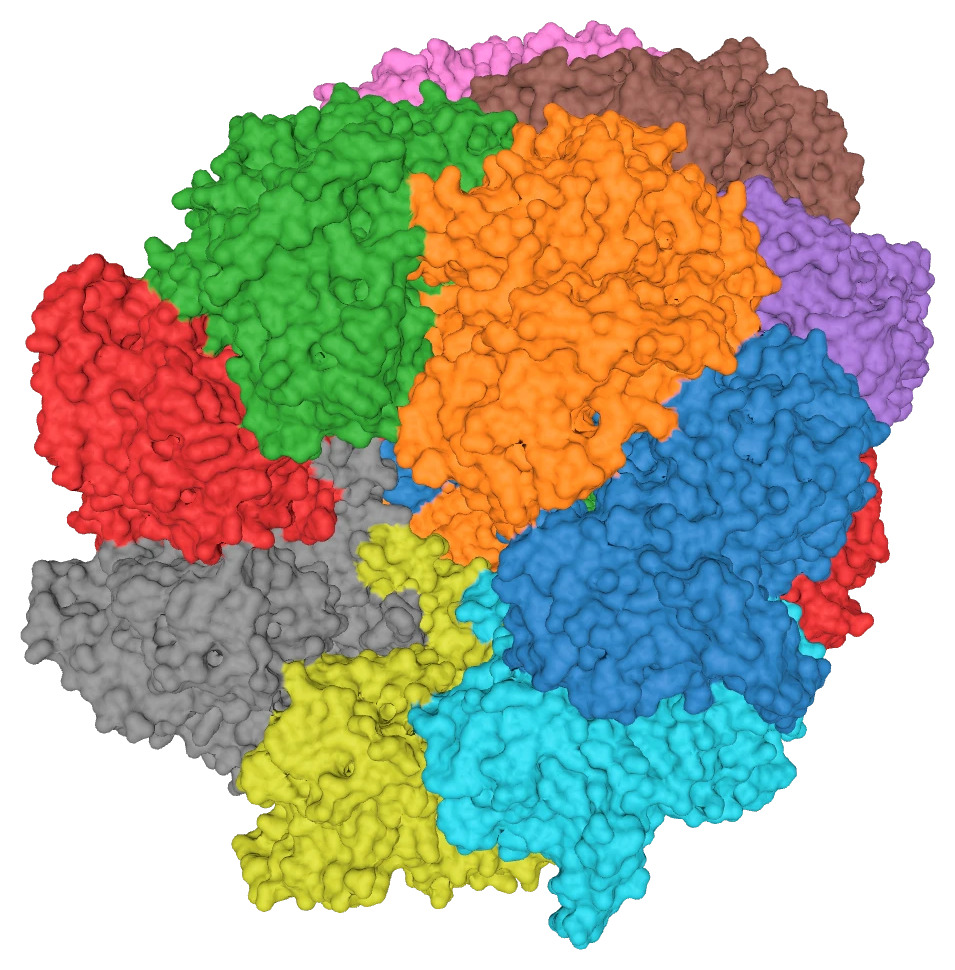
\includegraphics[width=\linewidth]{1aon-chain}
    \caption{1AON, by chain}
  \end{subfigure}\hfill
  \begin{subfigure}[b]{0.30\linewidth}
    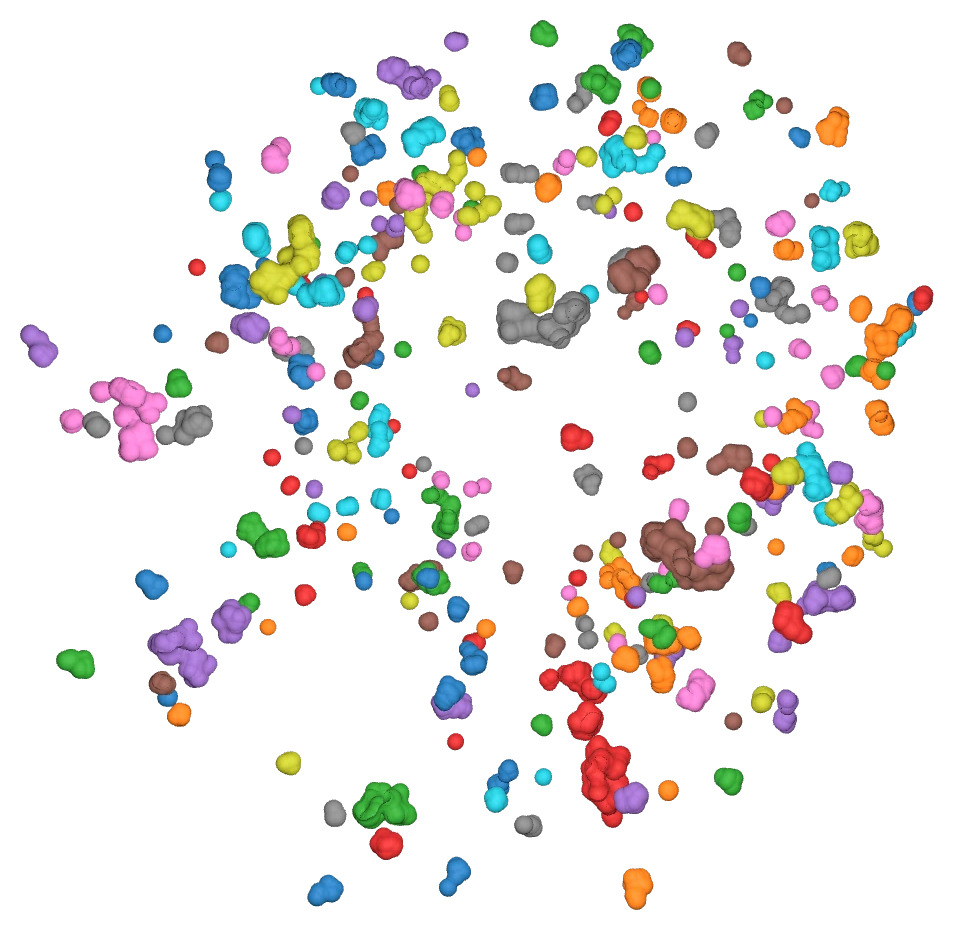
\includegraphics[width=\linewidth]{1aon-cavities}
    \caption{1AON cavities}
  \end{subfigure}\hfill
  \begin{subfigure}[b]{0.36\linewidth}
    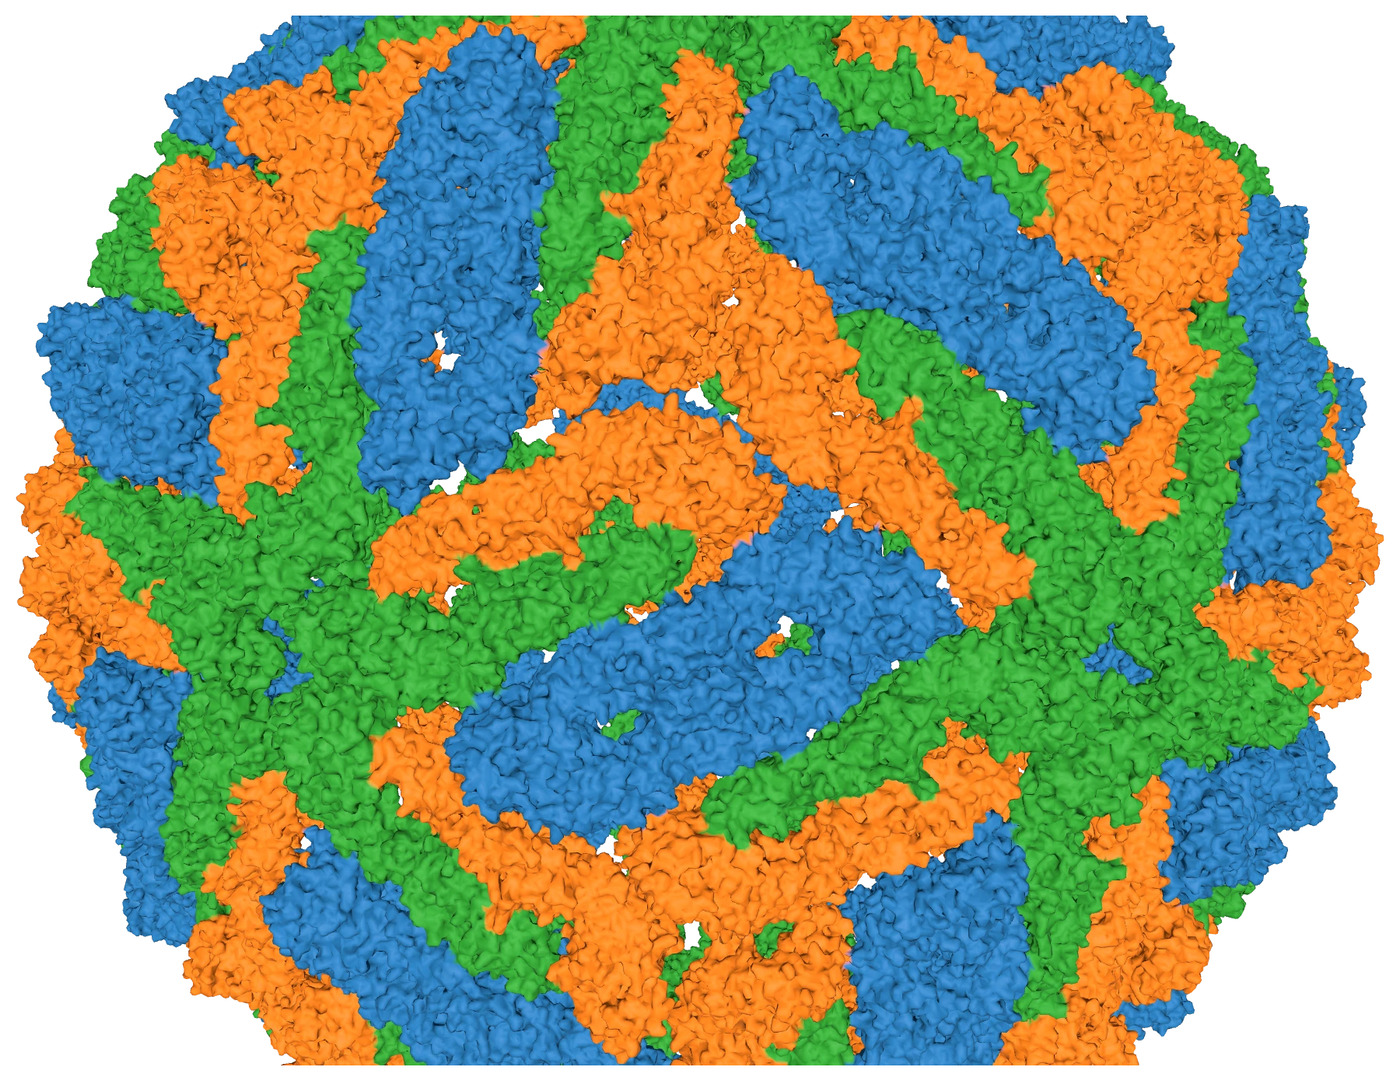
\includegraphics[width=\linewidth]{1k4r-capsid}
    \caption{1K4R capsid}
  \end{subfigure}
  \caption{(a)~GroEL--GroES (21 chains, 58\,870 atoms) at 0.5\Ang,
    decimated to 1.5\,M triangles. (b)~The same view showing only its 285
    internal cavities larger than 5\AA$^3$ (from a 0.25\Ang{} mesh), one
    colour each. (c)~Assembly~1 of the dengue virus capsid 1K4R, 60 copies
    of three envelope chains (545\,040 atoms) built from the file's
    operators, meshed at 1\Ang{} and decimated from 9.9\,M to 3\,M
    triangles for rendering.}
  \label{fig:gallery-large}
\end{figure}

% sesmesh — Solvent Excluded Surface meshes for molecules
% Copyright (c) 2026 Ugo Varetto
% SPDX-License-Identifier: MIT OR Apache-2.0

\section{Comparison with other programs}
\label{sec:comparison}

We compared \sesmesh{} 1.1.0 with five programs that produce SES meshes and
one that computes analytic SES areas (\cref{tab:cmp-programs}), on the
\val{corpus-n}-entry validation corpus at $h = 0.5$ and 0.25\Ang, the
\val{sweep-n}-entry random sweep at 0.5\Ang, nine degenerate synthetic
inputs and the benchmark set. Harness, container, raw data and the reference
numbers used by \sesmesh's tests are in the repository (\code{tools/compare},
\code{docs/validation/compare}, \code{tests/data/reference});
\code{docs/comparison.md} documents the protocol in full.

\begin{table}[t]
  \centering
  \caption{Programs compared. ``Same spheres'': the program accepts the
    atoms and radii used by \sesmesh{}; EDTSurf and sesa assign their own
    radii (sesa also adds hydrogens), so only their robustness, topology and
    speed compare directly.}
  \label{tab:cmp-programs}
  \footnotesize
  \setlength{\tabcolsep}{4pt}
  \begin{tabular}{@{}llp{0.40\linewidth}lc@{}}
    \toprule
    Program & Version & Method & Licence & Same spheres \\
    \midrule
    MSMS~\cite{sanner1996} & 2.6.2 (2026) & analytic reduced surface, template triangulation & non-commercial & yes \\
    NanoShaper~\cite{decherchi2013} & 0.7.5 & analytic patches, ray casting, Marching Cubes tables & GPL-3 & yes \\
    ESES~\cite{liu2017eses} & git 0b4cd51 & exact intersections on a Cartesian grid, Marching Cubes & none stated & yes \\
    ChimeraX~\cite{chimeraxsurface} & 1.12 (2026) & distance grid, contouring & non-commercial & yes \\
    EDTSurf~\cite{xu2009edtsurf} & 0.2009 & Euclidean distance transform, Marching Cubes & permissive & no \\
    sesa~\cite{wang2024sesa} & V001 & analytic SES area (no mesh) & GPL-3 & no \\
    \bottomrule
  \end{tabular}
\end{table}

\paragraph{Protocol.}
A helper writes the atoms and radii that \sesmesh{} uses by default (first
model, no hydrogens or waters, Bondi radii) in each program's input format,
with coordinates kept to three decimals as in the PDB archive and every atom
written as an \code{ATOM} record, because some programs skip or treat
\code{HETATM} ligands differently; for ChimeraX, which reads no PQR files,
the script sets every atom radius explicitly. Resolution is matched by the
grid spacing $h$ (grid scale $1/h$ for NanoShaper and EDTSurf, vertex density
$1.5/h^2$ for MSMS, from \cref{sec:density}). Cavities are kept everywhere
(MSMS \code{-all\_components}); NanoShaper runs without its optional mesh
smoothing, which moves vertices off the surface; ChimeraX builds one surface
around all atoms. A single checker reads every program's mesh and reports
its topology, area, signed volume and components, the distance of every
vertex to the exact SES of the same spheres, $|F(\vect v)|$, and the angle
between each vertex normal and the analytic normal. All runs used two
identical machines with an AMD Ryzen AI Max+ 395 (16 Zen~5 cores, SMT off,
128\,GB) and one Ubuntu 24.04 container holding every program; performance
runs had a machine to themselves.

\subsection{Accuracy}
\label{sec:cmp-accuracy}

NanoShaper and ESES construct the surface independently of \sesmesh{} and
also place their vertices on the exact SES, so they are the decisive
reference. At the same grid spacing their meshes agree with \sesmesh's to
within \val{cmp-nanoshaper-darea-max-0.25}\,\% (NanoShaper) and
\val{cmp-eses-darea-max-0.25}\,\% (ESES) in area and
\val{cmp-nanoshaper-dvol-max-0.25}\,\% and \val{cmp-eses-dvol-max-0.25}\,\%
in volume on every corpus entry at $h = 0.25$\Ang, and within
\val{cmp-nanoshaper-darea-max-0.5}\,\% and \val{cmp-eses-darea-max-0.5}\,\%
in area at 0.5\Ang{} (\cref{tab:cmp-accuracy}). All three are inscribed
meshes below the $h \to 0$ extrapolation by the same $O(h^2)$ amount, which
confirms the extrapolation of \cref{sec:proteins} with external references:
the specification's protein targets (area within 1\,\%, volume within
0.5\,\% at 0.25\Ang) hold against them.

MSMS's analytic SES area lies \val{cmp-msms-analytic-median}\,\% above the
extrapolation (median of \val{cmp-msms-analytic-n} entries; range
\val{cmp-msms-analytic-min} to \val{cmp-msms-analytic-max}\,\%), and its
mesh area scatters by up to \val{cmp-msms-area-worst-0.25}\,\%; the vertex
analysis below shows surface in the solvent region, which would have that
effect. ChimeraX's surfaces are smaller in area
(median \val{cmp-chimerax-area-med-0.5}\,\% at 0.5\Ang,
\val{cmp-chimerax-area-med-0.25}\,\% at 0.25\Ang) and larger in volume
(\val{cmp-chimerax-vol-med-0.5}\,\% and \val{cmp-chimerax-vol-med-0.25}\,\%).
EDTSurf's numbers refer to its own radii and are not listed.

\begin{table}[t]
  \centering
  \caption{Mesh area and volume relative to the $h \to 0$ extrapolation of
    each corpus entry (in \%, median and worst entry; same spheres). The
    last row is MSMS's analytic SES area (all components): median and
    range.}
  \label{tab:cmp-accuracy}
  \footnotesize
  \setlength{\tabcolsep}{4pt}
  \begin{tabular}{@{}lrrrrrrrr@{}}
    \toprule
    & \multicolumn{4}{c}{$h = 0.5$\Ang} & \multicolumn{4}{c}{$h = 0.25$\Ang} \\
    \cmidrule(lr){2-5}\cmidrule(l){6-9}
    & \multicolumn{2}{c}{area} & \multicolumn{2}{c}{volume} & \multicolumn{2}{c}{area} & \multicolumn{2}{c}{volume} \\
    Program & median & worst & median & worst & median & worst & median & worst \\
    \midrule
    \tablerows{generated/tab-cmp-accuracy.tex}
    \bottomrule
  \end{tabular}
\end{table}

\subsection{Vertices, normals and mesh validity}
\label{sec:cmp-validity}

\Cref{tab:cmp-validity} summarizes every run. \sesmesh, NanoShaper and ESES
wrote closed, consistently oriented, edge-manifold meshes in every run that
produced one; the median 99th-percentile vertex distance was
\val{cmp-p99-sesmesh}, \val{cmp-p99-nanoshaper} and \val{cmp-p99-eses}\Ang{}
respectively. NanoShaper still had a few vertices far from the surface on
some sweep entries (up to \val{cmp-worst-nanoshaper}\Ang).

\emph{MSMS} meshes had vertices more than 0.1\Ang{} from the SES in
\val{cmp-acc-off-msms} of \val{cmp-acc-meshed-msms} corpus runs and in
\val{cmp-sweep-off-msms} of \val{cmp-sweep-meshed-msms} sweep runs, up to
\val{cmp-worst-msms}\Ang; \val{cmp-acc-nm-msms} corpus and
\val{cmp-sweep-nm-msms} sweep meshes had non-manifold edges, mostly at the
higher density. On the small inhibitor 5PTI, for example, the worst MSMS
vertex has $F = +1.387$\Ang: it lies 0.013\Ang{} from a feasible probe
centre, i.e.\ in the solvent, which is consistent with concave patches of
overlapping probe positions not being clipped against each other. MSMS's
documentation also states that it restarts a failing computation up to five
times after enlarging the radii of the offending atoms by
0.1\Ang~\cite{msmsmanual}, which moves those parts of the surface.
\emph{ChimeraX} writes each patch with its own vertices, so none of its
meshes is closed as written (after merging coincident vertices nearly all
are), and its grid distances leave a median 99th-percentile vertex error of
\val{cmp-p99-chimerax}\Ang{} at 0.5\Ang. \emph{EDTSurf}'s vertices follow its
own radius model and are not comparable.

The checker also exposed a defect in \sesmesh{} 1.1.0 itself: on a few edges
where $F$ is not monotone (two concave patches meeting at a kink), the root
finder exhausted its evaluations and placed the vertex at an unevaluated
point, up to \val{cmp-worst-sesmesh}\Ang{} from the surface (one corpus
entry at 0.5\Ang{} and three sweep entries; at most 0.011\,\% of the
vertices of an affected mesh). This has since been fixed by bisecting such
edges, so every vertex is an evaluated point within $2.4\cdot10^{-5}$\Ang{}
of the SES away from the edge clamp \todo{name the release that contains the
fix (development branch \code{claude/intelligent-pasteur-0b9022}) and update
\cref{sec:refine,sec:analytic} accordingly}.

\begin{table}[t]
  \centering
  \caption{Robustness and mesh validity. Corpus: \val{corpus-n} entries at
    $h = 0.5$ and 0.25\Ang; sweep: \val{sweep-n} random PDB entries at
    0.5\Ang; synthetic: nine degenerate inputs. ``Closed'': closed,
    consistently oriented meshes as written, of those produced;
    ``n-m'': meshes with non-manifold edges; ``off'': meshes with a vertex
    more than 0.1\Ang{} from the exact SES (meaningful only for programs
    using the same spheres); last column: median 99th-percentile vertex
    distance on the corpus at 0.5\Ang.}
  \label{tab:cmp-validity}
  \footnotesize
  \setlength{\tabcolsep}{3pt}
  \begin{tabular}{@{}lrrrrrrrrrrrr@{}}
    \toprule
    & \multicolumn{5}{c}{Corpus} & \multicolumn{5}{c}{Sweep} & Synth. & \\
    \cmidrule(lr){2-6}\cmidrule(lr){7-11}\cmidrule(lr){12-12}
    Program & runs & failed & closed & n-m & off & runs & failed & closed & n-m & off & failed & p99 (\AA) \\
    \midrule
    \tablerows{generated/tab-cmp-validity.tex}
    \bottomrule
  \end{tabular}
\end{table}

\subsection{Cavities}
\label{sec:cmp-cavities}

Trypsin (2PTN), the case of issue \#6, has \val{cmp-2ptn-sesmesh-0.25}
cavities in \sesmesh, NanoShaper and ESES at both spacings, with the same
total volume to 0.1\AA$^3$; MSMS reports \val{cmp-2ptn-msms-0.25} and
ChimeraX \val{cmp-2ptn-chimerax-0.25} at 0.25\Ang. Over the corpus
(\cref{tab:cmp-cavities}), cavities found by NanoShaper or ESES but not
matched by a \sesmesh{} cavity have their vertices on the exact SES (median
distance $\le 10^{-3}$\Ang): they are the same cavity space split or joined
differently at necks thinner than the grid, and their number falls sharply
from 0.5 to 0.25\Ang. MSMS reports about twice as many cavities as the
three exact-vertex methods, and half of its unmatched ones have vertices
0.5\Ang{} or more from the SES. The C$_{60}$ fullerene of NanoShaper's
examples has one internal cavity in \sesmesh, NanoShaper, ESES and ChimeraX
and none in MSMS, as Decherchi and Rocchia reported~\cite{decherchi2013}.

\begin{table}[t]
  \centering
  \caption{Cavities (closed components of negative volume) on the corpus,
    matched to \sesmesh's cavities by centroid within 1\Ang. ``Max dist'':
    median over unmatched cavities of their largest vertex distance to the
    exact SES.}
  \label{tab:cmp-cavities}
  \footnotesize
  \begin{tabular}{@{}lrrrrrr@{}}
    \toprule
    Program & $h$ (\AA) & cavities & \sesmesh{} cavities & unmatched & max dist (\AA) & \sesmesh{} not found \\
    \midrule
    \tablerows{generated/tab-cmp-cavities.tex}
    \bottomrule
  \end{tabular}
\end{table}

\subsection{Robustness and determinism}
\label{sec:cmp-robustness}

\sesmesh{} produced a valid mesh for every input. MSMS failed on
\val{cmp-sweep-fail-msms} of \val{cmp-sweep-runs-msms} sweep entries, on the
ribosomal subunit 1FFK at both densities (after its radius-enlarging
restarts) and on the 2.44-million-atom HIV-1 capsid 3J3Q; Goddard reported
that earlier MSMS versions crash on most structures above 10\,000
atoms~\cite{goddard2013}, and version 2.6.2 lists many such crashes as
fixed. NanoShaper crashed (segmentation fault) on the 80S ribosome 4V6X at
4 grid points per \AA{}, also with five-fold larger acceleration-grid limits,
and stopped with an error status and no message on 3J3Q at 1\Ang{} and on
the one- and two-atom synthetic inputs. ESES crashed on the input placed
$10^4$\Ang{} from the origin and misplaced vertices by up to 1.3\Ang{} on
exact duplicate atoms; ChimeraX also failed on the offset input. EDTSurf
aborted on both capsids at 1\Ang, and sesa crashed on 3J3Q. Memory sets the
other limits: ESES needed 21\,GiB for 1AON at 0.25\Ang{} and 42\,GiB for
3J3Q at 1\Ang, and was stopped at a 40\,GiB cap on 4V6X at 0.25\Ang; MSMS
needed 47\,GiB for the 1K4R capsid.

Outputs were compared byte for byte (ignoring comment lines, since
NanoShaper writes a date into its header) for 1, 2, 4, 8 and 16 threads and
repeated runs on 4HHB and 1AON. \sesmesh, NanoShaper and ChimeraX produced
identical files at every thread count, MSMS and EDTSurf (single-threaded)
across repeats; ESES's output for 1AON differed at every thread count.

\subsection{Performance}
\label{sec:cmp-performance}

\Cref{tab:cmp-perf} lists wall time and peak memory on the benchmark set,
with all 16 cores available to the multi-threaded programs. \sesmesh{},
ESES and ChimeraX completed every entry; NanoShaper, MSMS and EDTSurf
failed on the largest. \sesmesh{} was the fastest program on every entry at
matched resolution: NanoShaper took \val{ratio-nanoshaper-min} to
\val{ratio-nanoshaper-max} times as long (median
\val{ratio-nanoshaper-med}), ChimeraX \val{ratio-chimerax-min} to
\val{ratio-chimerax-max} times, ESES \val{ratio-eses-min} to
\val{ratio-eses-max} times, and single-threaded MSMS \val{ratio-msms-min}
to \val{ratio-msms-max} times; the median memory ratios are
\val{memratio-nanoshaper-med} (NanoShaper), \val{memratio-chimerax-med}
(ChimeraX), \val{memratio-eses-med} (ESES) and \val{memratio-msms-med}
(MSMS). EDTSurf is faster on 1AON at 0.25\Ang, but its grid does not
reach the requested resolution on large molecules: it produced
\val{tri-edtsurf-1AON-0.25}\,M triangles there, against
\val{tri-sesmesh-1AON-0.25}\,M for \sesmesh.

\begin{table}[t]
  \centering
  \caption{Wall time in seconds (peak memory in GiB) of complete runs on one
    16-core Zen~5 machine; median of three runs where repeated. Each program
    writes its own output format; ESES also writes many auxiliary files.
    \sesmesh, NanoShaper, ESES and ChimeraX use 16 threads; MSMS, EDTSurf
    and sesa are single-threaded; sesa computes areas only, with its own
    radii, independent of $h$. ``fail'': crash or error.}
  \label{tab:cmp-perf}
  \footnotesize
  \setlength{\tabcolsep}{3pt}
  \begin{tabular}{@{}lrrrrrrrr@{}}
    \toprule
    Entry & $h$ & \sesmesh{} & NanoShaper & ESES & MSMS & ChimeraX & EDTSurf & sesa \\
    \midrule
    \tablerows{generated/tab-cmp-perf.tex}
    \bottomrule
  \end{tabular}
\end{table}

\paragraph{Limitations of the comparison.}
All timings come from one machine type, with the programs' default build
options; settings that trade accuracy for speed (MSMS density, NanoShaper's
grid scale) were matched to \sesmesh's resolution rather than tuned per
program. The programs write different output formats, which is part of
their cost. EDTSurf and sesa cannot use the same radii. sesx, the exact
triangulator by the author of sesa, is an interactive viewer without mesh
export, and GPU programs~\cite{hermosilla2017,martinez2019quickses} are
outside the scope of a CPU comparison.

% sesmesh — Solvent Excluded Surface meshes for molecules
% Copyright (c) 2026 Ugo Varetto
% SPDX-License-Identifier: MIT OR Apache-2.0

\section{Discussion and limitations}
\label{sec:discussion}

\paragraph{What exactness buys.}
Sampling the exact field changes the error budget of a grid method:
vertices lie on the SES to within $10^{-4}h$ and normals are exact, so the
only discretization error left is that of a piecewise-linear surface
through exact points, which decreases as $O(h^2)$ with a small constant.
On the same spheres and grid, the mean area error at the default 0.5\Ang{}
grid (\val{area-mean-0.5}\,\%) compares with
\val{cmp-chimerax-area-med-0.5}\,\% for ChimeraX's distance grid, and two
independent exact-vertex programs, NanoShaper and ESES, reproduce \sesmesh's
areas and volumes to a few hundredths of a per cent
(\cref{sec:comparison}). Because classification is conservative and the
table is uniform, the same code path yields closed manifold meshes for
every input tried, without perturbation or restarts. Exactness also makes
the mesh testable: measuring every vertex against the exact field revealed
both other programs' defects and a rare root-finding failure in \sesmesh{}
1.1.0 (\cref{sec:cmp-validity}).

\paragraph{Limitations.}
\begin{itemize}
  \item \emph{Inscribed meshes underestimate area} (by
    \val{area-mean-0.25}\,\% on average at 0.25\Ang{} for proteins, and by
    up to \val{an-area-hi-0.25}\,\% for the atom-sized analytic
    references). Applications that need the area itself
    should use a finer grid or the $h \to 0$ extrapolation; an analytic
    area and volume in the style of Quan and Stamm or sesa is future
    work~\cite{quan2016,wang2024sesa}.
  \item \emph{Topology at coarse spacing.} The uniform face rule guarantees
    manifoldness, not the topology of the trilinear interpolant
    (MC33~\cite{lewiner2003,custodio2013}). Features thinner than $h$ can
    be cut off as sub-grid fragments (\cref{sec:fragments}) or, by the
    same mechanism, thin necks can be merged or split; such fragments are
    identified exactly and can be dropped, but other topological changes
    below the grid resolution are not detected.
  \item \emph{Uniform resolution.} The grid spacing is uniform; decimation
    redistributes triangles afterwards, but there is no curvature-adaptive
    sampling.
  \item \emph{Exactly fitting probes} (a probe that fits a cavity exactly)
    are decided by a fixed tolerance of $10^{-9}$\Ang; the result is
    deterministic but, like any such decision, arbitrary at the tie.
  \item \emph{Memory per atom.} The exact double-precision arrangement
    costs about 560 bytes per atom; a 545\,000-atom capsid needs about
    640\,MiB for its atoms alone, so very tight memory limits force very
    coarse grids (6.1\Ang{} under 700\,MiB).
  \item \emph{Determinism scope.} Byte-identical output holds for the same
    binary and SIMD level. Across SIMD levels, sampled field values agree
    within $2\cdot10^{-5}$\Ang{} in the tests, so the mesh topology can
    differ only at samples that close to the surface.
\end{itemize}

\paragraph{Open measurements.}
Still missing: (i)~timings on the specification's Apple Silicon reference
machine with 8 performance cores (the x86-64 measurements of
\cref{sec:x86} cover the homogeneous-core case); (ii)~a robustness sweep of
1\,000 rather than 200 entries; and (iii)~a fuzzing campaign of at least
24 CPU-hours per parser, of which only 10 minutes per target have been run
\todo{update this paragraph as each item is completed}.

\paragraph{Future work.}
The brick and structure-of-arrays kernel design maps directly to GPU
compute; other planned extensions are MC33 and dual
meshers~\cite{gibson1998,ju2002}, adaptive resolution, analytic area and
volume, Gaussian and skin surfaces as further field kinds, region-restricted
surfaces (for example a binding pocket), Python bindings and a WebAssembly
build.

% sesmesh — Solvent Excluded Surface meshes for molecules
% Copyright (c) 2026 Ugo Varetto
% SPDX-License-Identifier: MIT OR Apache-2.0

\section{Availability}
\label{sec:availability}

\begin{center}
\small
\begin{tabular}{@{}>{\bfseries}l p{0.7\linewidth}@{}}
  Software & \sesmesh{} 1.1.0, released 2026-11-14 (first public release
    0.9.0 and 1.0.0 on 2026-11-13); library crate \code{sesmesh}, command-line
    crate \code{sesmesh-cli} (binary \code{sesmesh})~\cite{sesmesh} \\
  Source code & \url{https://github.com/uvar-apps/sesmesh} \\
  Packages & \url{https://crates.io/crates/sesmesh},
    \url{https://crates.io/crates/sesmesh-cli};
    API documentation at \url{https://docs.rs/sesmesh} \\
  Binaries & GitHub releases for macOS arm64, Linux x86-64 and arm64,
    Windows x86-64 \\
  Website & \url{https://uvar-apps.github.io/sesmesh/} (guides, tutorials,
    gallery, interactive viewer) \\
  Archive & Zenodo, DOI \todo{mint a Zenodo DOI for v1.1.0 (or the version
    the paper describes) and cite it here and in \code{CITATION.cff}} \\
  Licence & MIT or Apache-2.0, at the user's option \\
  Language & Rust 1.89 or newer; no unsafe code; dependencies from
    crates.io only \\
  Install & \code{cargo install sesmesh-cli}; library: \code{sesmesh = "1"}
    in \code{Cargo.toml} \\
\end{tabular}
\end{center}

\paragraph{Data and reproducibility.}
The validation data used in this paper are in the repository
(\code{docs/validation/}: accuracy study, robustness sweep, large inputs),
together with the commands that regenerate them. Structures are fetched from
the RCSB PDB by \code{cargo xtask fetch}, whose lock file pins their SHA-256
checksums; PDB data are in the public domain (CC0). The paper's sources,
figures, the script that turns the data into its tables and plots, and the
program that produces the analytic-reference data are in \code{paper/}
(\cref{app:reproduce}).

\section*{Declarations}

\paragraph{Use of AI tools.}
\todo{Author to review and finalize this statement, and check it against
the target venue's policy.} The software, its tests and documentation,
and a first draft of this manuscript were developed with the help of an AI
coding assistant (Anthropic's Claude Opus 5.5, used through Claude Code).
Commits to which the assistant contributed carry a
\code{Co-Authored-By: Claude} trailer in the project's version history
(30 of the 31 commits at the time of writing). The author designed and directed
the work, reviewed the code, the measurements and the text, and takes full
responsibility for the content.

\paragraph{Competing interests.}
\todo{Confirm: the author declares no competing interests.}

\paragraph{Funding.}
\todo{Funding statement, or ``This work received no specific funding.''}

\paragraph{Author contributions.}
\todo{CRediT statement if the venue requires one; single author.}

\paragraph{Acknowledgements.}
\todo{Acknowledgements, if any.} The atomic coordinates used in this work
were obtained from the Protein Data Bank \todo{cite the RCSB PDB / wwPDB
reference recommended by the archive}.


\bibliographystyle{unsrtnat}
\bibliography{references}

\appendix
% sesmesh — Solvent Excluded Surface meshes for molecules
% Copyright (c) 2026 Ugo Varetto
% SPDX-License-Identifier: MIT OR Apache-2.0

\section{Validation corpus}
\label{app:corpus}

\Cref{tab:corpus} lists the \val{corpus-n} entries of the accuracy study
of \cref{sec:proteins} with their results at $h = 0.25$\Ang{} and the area
and volume errors at 0.5\Ang. $A_0$ is the $h \to 0$ extrapolation of the
area. Components include cavities and, in this data set (made with
version 1.0.0), the sub-grid fragments of \cref{sec:fragments}. Times are
those of the meshing call alone on the loaded 10-core machine.

{\small
\setlength{\tabcolsep}{4pt}
\begin{longtable}{@{}lrrrrrrrrr@{}}
  \caption{Validation corpus at $h = 0.25$\Ang{} (errors in \%; generated
    from \code{docs/validation/accuracy.csv}).}\label{tab:corpus}\\
  \toprule
  & & & & & \multicolumn{2}{c}{Area error} & \multicolumn{2}{c}{Volume error} & \\
  \cmidrule(lr){6-7}\cmidrule(lr){8-9}
  Entry & Atoms & Triangles & Cavities & $A_0$ (\AA$^2$) & 0.5\Ang & 0.25\Ang &
    0.5\Ang & 0.25\Ang & Time (s) \\
  \midrule
  \endfirsthead
  \toprule
  Entry & Atoms & Triangles & Cavities & $A_0$ (\AA$^2$) & 0.5\Ang & 0.25\Ang &
    0.5\Ang & 0.25\Ang & Time (s) \\
  \midrule
  \endhead
  \bottomrule
  \endfoot
  \tablerows{generated/tab-corpus.tex}
\end{longtable}
}

\section{Reproducing the data in this paper}
\label{app:reproduce}

From a checkout of the repository at the release tag \todo{tag or commit
the final paper refers to}:

\begin{lstlisting}
cargo xtask fetch --set validation --set sweep --set bench   # PDB entries (~70 MB)
cargo run --release -p xtask -- validate     # docs/validation/accuracy.csv
cargo run --release -p xtask -- sweep        # docs/validation/sweep.csv
cargo build --release                        # target/release/sesmesh
/usr/bin/time -l target/release/sesmesh tests/data/cache/3J3Q.cif.gz -s 1.0 \
    -o /dev/null --stats /dev/stdout         # large inputs (time, peak RSS)
cd paper && make                             # analytic data, tables, plots, PDF
\end{lstlisting}

\noindent The analytic data (\code{paper/\allowbreak data/\allowbreak analytic.csv})
come from a small program in \code{paper/\allowbreak scripts/\allowbreak analytic}
that links the library and the analytic references of its test kit;
\code{paper/\allowbreak scripts/\allowbreak make\_data.py}
(Python~3 standard library only) turns the CSV files into the tables, the
\code{\textbackslash val\{\}} numbers in the text and the data of the plots.
The thread-scaling data (\code{paper/data/scaling.csv}) are transcribed from
the design document, and the timings of \cref{tab:perf} and the 1.1.0 memory
figures of \cref{tab:large} from the validation report.


\ifshowtodos
\clearpage
\listoftodos
\fi

\end{document}
